\section{Introduction}

\begin{figure}
  \begin{center}
    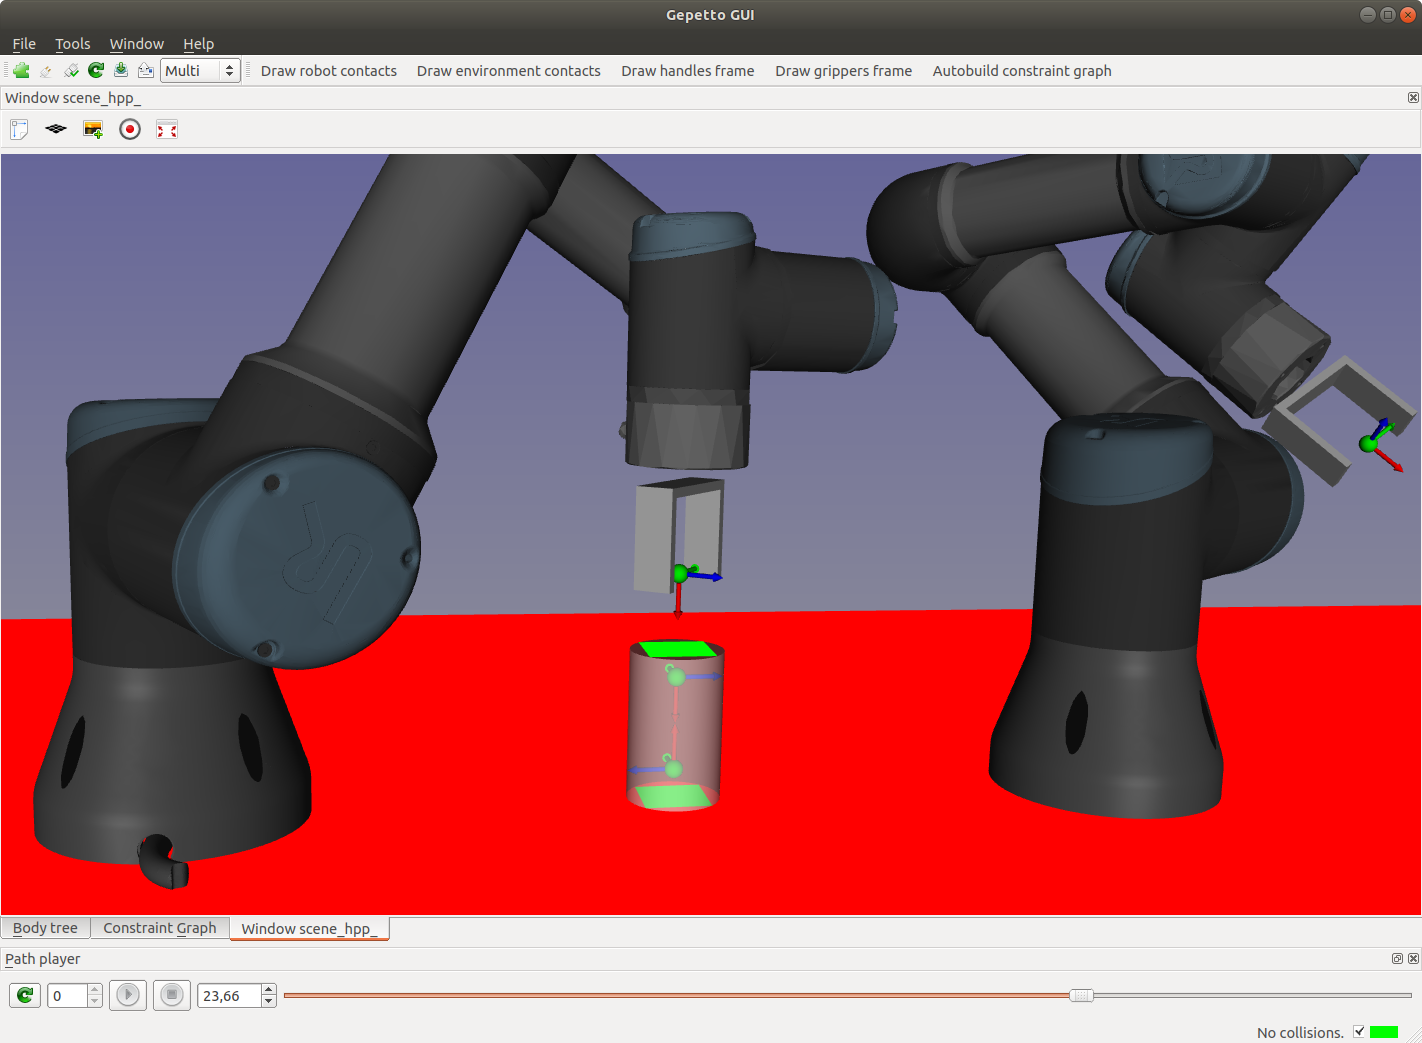
\includegraphics[width=\linewidth]{figures/example.png}
    \def\svgwidth{\columnwidth}
    \graphicspath{{./figures/}}
    \input{figures/example-graph.pdf_tex}
  \end{center}
  \caption{{\color{blue} Example of manipulation planning problem.} Top: two UR3 robots with one gripper each (X=red, Y=green, Z=blue) manipulating a cylinder with two handles. The environment contains one rectangular contact surface (in red). The cylinder has two rectangular contact surfaces (in green).
  Bottom: the corresponding constraint graph. Names of states follow Expression~(\ref{eq:state}): for example, $(\emptyset,1)$ means that gripper of robot 2 grasps handle 1 of the cylinder. In this state, there is no placement constraint.}
  \label{fig:2ur3-cylinder}
\end{figure}

Today, robots in industrial manufacturing are mostly programmed by
hand. They repeat the same motion thousands of times with a high
accuracy. However, automating a task with some variability is very
challenging since it requires more programming effort to integrate
sensors and motion planning in the process. A good example of this difficulty is
the Amazon picking challenge \cite{brock-2018}. The work described in this
paper is a small step to the simplification of industrial process
automation in the presence of some variability, like the variation of
the initial position of some object or the presence of unknown
obstacles. The work only covers the motion planning -- and
more accurately the manipulation planning -- issue. The integration in a whole
process is still under development. We think that it
is important not only to develop algorithms, but also to provide them
within an open-source software platform in order to make the
evaluation and then the integration of those algorithms easier.

Therefore this \paper describes a software platform called {Humanoid Path
  Planner} tailored for manipulation planning in robotics. It can handle many types of robots, from manipulator arms to legged humanoid robots.
The main contributions are:
\begin{itemize}
\item an original and general modelling of prehensile manipulation based on
  nonlinear constraints,
\item an original solver for nonlinear constraints that is able to handle implicit and explicit constraints,
\item a manipulation planning algorithm that is able to tackle a great variety of manipulation planning problems,
\item an open-source software suite that implements all the above following state-of-the-art development tools and methods.
\item a docker image of the aforementioned software with installation instructions provided with this paper. This image makes the experimental results replicable.
\end{itemize}
{\color{blue} Installation instructions can be found by following this \href{https://humanoid-path-planner.github.io/hpp-doc}{link}.}
This paper extends the work presented in {\color{blue} previous papers }\cite{mirabel-iros2016},\cite{MirLam2018} with the following new material:
\begin{itemize}
\item description of the configuration space as a Cartesian product of Lie groups (Section~\ref{partie:preliminary}),
\item unified and detailed definition of the grasp and placement constraints that are only evoked in {\color{blue}Mirabel \textit{et al}}~\cite{mirabel-iros2016} (Section~\ref{sec:manipulation-problem}),
\item automatic construction of the constraint graph (Section~\ref{sec:manipulation-problem}),
\item the docker image of the software,
\item a description of the software platform (Section~\ref{sec:humanoid-path-planner}),
\item experimental results on several different problems.
\end{itemize}

The \paper is organized as follows. \Partie~\ref{sec:related-work} presents some related work for constrained motion planning and manipulation planning.
\Partie~\ref{partie:preliminary} introduces some preliminary notions like kinematic chains and Lie groups that are used to model the configuration space of each joint. \Partie~\ref{sec:constraints} introduces nonlinear constraints and solvers that are at the core of manipulation problem definition. \Partie~\ref{sec:manipulation-problem} defines the problem of prehensile manipulation in the general setting. \Partie~\ref{sec:manipulation-planning} provides a general algorithm that solves manipulation planning problems. Finally, \partie~\ref{sec:humanoid-path-planner} is devoted to the software platform implementing the notions introduced in the previous sections. Experimental results are provided for a large variety of problems.

Each \partie is implemented by one or several software packages. For some values that need to be computed, instead of providing formulas, we sometimes provide a link to the C++ or python implementation.

\section{Related work}\label{sec:related-work}

Motion planning has given rise to a lot of research work for the past decades.
The problem consists in finding a collision-free path for a given system in
an environment populated with obstacles. The field covers a large variety of
different applications ranging from navigation for autonomous vehicles in
partially known environments~\cite{DarpaUrbanChallenge} to path planning for
deformable objects~\cite{LamKav2001}, \cite{RouFerTai2020} and many other applications like coverage path planning~\cite{coverage2001}, \cite{coverage2013}, or pursuit evasion planning~\cite{pursuit-evasion1999}.

Planning motions for high dimensional robots like humanoid robots or multi-arm
systems has been proven to be of a very high complexity~\cite{SchSha1983}, \cite{Canny1983}. Starting in the 1990's random sampling methods have been proposed
to solve the problem, trading the completeness property against efficiency in
solving problems in high dimensional configuration spaces \cite{KSLO1996}, \cite{HsuLatMot99}, \cite{KufLav00}. The latter methods are said probabilistically complete since the probability to find a solution if one exists converges to 1 when the time of computation tends to infinity. Since then, asymptotically optimal random sampling algorithms have
been proposed~\cite{KarFra2011}.

\subsection{Path planning with nonlinear constraints}

Some systems are subject to nonlinear constraints. These nonlinear
constraints define sub-manifolds of the configuration space the robot
must stay on. For example, legged robots that must keep contact with
the ground and enforce quasi-static equilibrium, or multi-arm systems
grasping a same object are subject to this type of constraints. As the
volume of the constrained manifold is usually equal to zero, sampling
random configurations satisfying the constraints is an event of zero
probability. To sample configurations on the constrained manifold,
{\color{blue}Dalibard \textit{et al}}~\cite{DalNakLamLau2009} and {\color{blue}Benrenson
\textit{et al}}~\cite{berenson2011} project random configurations using
a generalization of Newton-Raphson algorithm. Another way to sample
configurations on a constrained manifold consists in expressing some
configuration variables with respect to others~\cite{Cortes2002},
\cite{MirLam2018} whenever this is possible. {\color{blue}Jaillet \textit{et al}}~\cite{atlasRRT} propose
another method based on nonlinear projection. They cover the
constrained manifold by growing an atlas composed of local
charts. This approximation provides a probability distribution that is
closer to the uniform distribution over the manifold than the
projection of a uniform distribution over the configuration
space. {\color{blue}Beobkyoon \textit{et al}}~\cite{tb-rrt2016} propose a variation of the latter paper.  The
main difference resides in the fact that the nodes built on the
tangent space are not immediately projected on the manifold.
{\color{blue}Cefalo \textit{et al}}~\cite{CefOri2019} propose a general framework to plan task constrained
motions in the presence of moving obstacle. {\color{blue}Kingston \textit{et al}}~\cite{KinMolKav2019}
provide an in-depth review of the various approaches to motion
planning with nonlinear constraints.

\subsection{Manipulation planning}

Manipulation planning is a particular instance of path planning where
some objects are moved by some robots.
Although several instances of the
manipulation problem exist like manipulation by
pushing~\cite{BenRiv1998}, or by throwing~\cite{WooZacLyn2017}, as well as
multi-contact planning \cite{Bretl2006}, \cite{LenVaiYosKhe2013},
\cite{TonDelPetParManMan2018}, in this paper, we are only concerned with
prehensile manipulation.
The configuration space of the whole system is constrained by
nonlinear constraints due to the fact that objects cannot move by
themselves and should stay in a stable pose when not grasped by a
robot.  The accessible configuration space is thus a union of
sub-manifolds as defined in the previous section. Each of these
manifolds may moreover be a foliation where each leaf corresponds to a
stable pose of an object or to a grasp of an object by a
gripper. The geometrical structure of the problem has been well
understood for a long time~\cite{AlaSimLau89}. Some specific instances of the
problem have even been addressed recently \cite{vendittelli-2018}.

The first attempt to solve manipulation planning problems using random sampling
was proposed by {\color{blue}Siméon \textit{et al}}~\cite{simeon2004ijrr} where a reduction property reduces the
complexity of the problem.

Papers about manipulation planning are commonly divided into several categories.

Navigation Among Movable Obstacles (NAMO) \cite{wilfong1988motion}, \cite{stilman2008planning} consists in finding
a path for a robot that needs to move objects in order to reach a goal
configuration. The final poses of the objects do not matter in this case.

Rearrangement planning \cite{ota2004rearrangement}, \cite{LIS210},
\cite{KroBek2015}, \cite{LerPha2015} consists in finding a sequence of
manipulation paths that move some objects from an initial pose to a
final pose. The final configuration of the robot is not specified. A
simplifying assumption is the existence of a monotone solution, that is
a solution where each object is grasped at the most once and is moved from
its initial pose to its final pose \cite{stilman2008planning},
\cite{stilman2007manipulation}, \cite{srivastavaetal2014icra}, \cite{nieuwenhuisen2008effective},
\cite{ota2004rearrangement}. They mostly use two-level methods
composed of a symbolic or task planner and of a motion
planner~\cite{cambon:hal-01976081}, \cite{KaeLoz2013}, \cite{LozKae2014}, \cite{18-toussaint-RSS}.

Other contributions in manipulation planning explicitly address the problem of multi-arm manipulation \cite{GhaCorSim2009}, \cite{HarTsuLau2014}, \cite{DobBek2015}, \cite{XiaLerPha2017}.

{\color{blue}Schmitt \textit{et al}}~\cite{schmitt19icra} propose an approach where two robots manipulate an object in a dynamic environment. The output of the algorithm is a sequence of controllers rather than a sequence of paths.

Our work shares many ideas with {\color{blue}Hauser and Ng-Thow-Hing} \cite{HauNgt2011} where the notion of constraint
graph is present, although not as clearly expressed as in this paper. The main
contribution of our work with respect to the latter paper is that the
constraint graph is built automatically at the cost of a more restricted range
of applications. We address indeed only prehensile manipulation.

\subsection{Open-source software platforms}

Open-source software platforms are an important tool to make possible fair
comparison between algorithms.
Several software platforms are available for motion planning and/or manipulation
planning in the robotics community. The most popular one is undoubtedly OMPL \cite{ompl2012}. OMPL integrates many randomized path planning algorithms and is widely used for teaching. Recently, {\color{blue}Kingston \textit{et al}}~\cite{KinMolKav2019} proposed an extension for systems subject to nonlinear constraints.

OpenRave~\cite{diankov_thesis} is
a software platform that addresses motion and manipulation planning. It includes
computation of forward kinematics.

One of the main differences between our solution and the previously cited ones resides in the way manipulation constraints are compiled into a graph. To our knowledge none of the previous solutions can handle a variety of problems as large as those described in Section~\ref{sec:benchmarks}.

\section{Preliminaries: kinematic chains and Lie groups}\label{partie:preliminary}

A kinematic chain is commonly understood as a set of rigid-body links connected
to each other by joints. Each joint has one degree of freedom either in
rotation or in translation. A configuration of the kinematic chain is represented by a vector. Each component of the vector represents the angular or linear value of the corresponding joint.

This representation although well suited for fixed base manipulator
arms is not well adapted for robots with a mobile base like wheeled
mobile robots, aerial robots or legged robots, since the mobility of the base
cannot be correctly represented by translation or rotation joints.
Representing a free-flying object by three virtual translations followed by
three virtual rotations called roll, pitch and yaw is indeed a poor workaround
due to the presence of singularities. A good illustration of this is the gimball
lock issue that arose during Apollo~13 flight. To avoid singularities, we
propose the following definition.

\subsubsection{Kinematic chain}

A \textit{kinematic chain} is a tree of \textit{joints} where each
joint represents a mobility of a rigid-body link with respect to
another link or with respect to the world reference frame. To each joint is
associated a configuration space called the \textit{joint configuration space}.
The most common joints with their respective configuration spaces are
\begin{itemize}
\item linear \textit{translation} with configuration space $\reals$,
\item bounded \textit{rotation} with configuration space  $\reals$,
\item unbounded \textit{rotation} with configuration space  $SO(2)$,
\item \textit{planar} joint with configuration space $SE(2)$,
\item \textit{freeflyer} joint with configuration space $SE(3)$.
\end{itemize}
$SO(n)$ and $SE(n)$ respectively stand for \textit{special orthogonal group} and \textit{special Euclidean group}. They represent the group of rotations and the group of rigid-body transformations in $\reals^n$.

\subsubsection{Lie groups}

The joint configuration spaces enumerated in the previous paragraph: $\mathbb{R}^n$, $SO(n)$, and $SE(n)$ are all Lie groups. The group operation is $+$ for $\mathbb{R}^n$, and composition denoted as $"."$ for $SE(n)$. We refer to~{\color{blue}Murray \textit{et al}}~\cite[Appendix A]{LMS94} for a thorough definition of Lie groups. Here we detail only properties that are useful for the following developments.

For any Lie group $\liegroup$ with neutral element $\neutral$, the tangent space at the neutral element $T_{\neutral}\liegroup$ of the group naturally maps to the tangent space at any point of the group. This means that any \textit{velocity} $\mathbf{v}\in T_{\neutral}\liegroup$ uniquely defines
\begin{enumerate}
\item a velocity $\mathbf{w}\in T_{g}\liegroup$ at any point $g$ of the group, and thus,
\item a vector field on the tangent space $T\liegroup$, and
\item by integration during unit time of the latter vector field, starting from the origin, a new point $g_{1}\in\liegroup$.
\end{enumerate}
Item 1 above is called the \textit{transport} of velocity $\mathbf{v}$ to $g$.
Item 3 is called the exponential map of $\liegroup$ and is denoted by $\exp$.

\paragraph{Geometric interpretations}
\begin{itemize}
\item $\reals$ (and by trivial generalization $\reals^n$): the neutral element is $0$. The tangent space at 0 is isomorphic to $\reals$ and
  $$
  \forall \theta\in\reals,\  \exp(\theta) = \theta.
  $$
\item $SE(3)$: an element $g$ of $SE(3)$ can be seen as the position of a moving frame in a fixed reference frame. A point $\mathbf{x}\in\reals^3$ is mapped to $g(\mathbf{x})$. Note that $\mathbf{x}$ is also the coordinate vector of $g(\mathbf{x})$ in the moving frame $g$. If $\mathbf{v}$, $\omega$ are a linear and an angular velocities at the origin, $(\mathbf{v},\omega)$ is \textit{transported} to $g$
  as the same linear and angular velocities expressed in the moving frame. In other words, if
  \begin{equation}\label{eq:homogeneous matrix}
  M=\left(\begin{array}{ll} R & \mathbf{t}\\ 0 & 1\end{array}\right)
    \end{equation}
  with $R\in SO(3)$ and $\mathbf{t}\in\reals^3$  is the homogeneous matrix
  representing $g$, and $(\mathbf{v},\mathbf{\omega})$ is a velocity in $T_{I_3}SE(3)$, the velocity \textit{transported} to $g$ corresponds to linear and angular velocities $R\mathbf{v}$ and $R\omega$ of the moving frame.
  Integral curves of the vector field mentioned in item 2 above correspond to screw motions of constant velocity expressed in the moving frame.
\end{itemize}
$SE(2)$, $SO(3)$, and $SO(2)$ are (or are isomorphic to) subgroups of $SE(3)$ and follow the same geometrical interpretation.

\paragraph{Vector representations}
Each Lie group element is represented by a vector. Rotations are represented by
unit quaternions.

Therefore elements of $SE(3)$ are represented by a vector in $\reals^7$ where the first 3 components represent the image of the origin (vector $\mathbf{t}$ in Equation~\ref{eq:homogeneous matrix}), the last 4 components $(x,y,z,w)$ represent unit quaternion $w + x {i} + y {j} + z {k}$.

Elements of $SO(3)$ are likewise represented by a unit vector of dimension 4.

Elements of $SE(2)$ are represented by a vector of dimension 4. The first 2 components represent the image of the origin. The last 2 components represent the cosine and sine of the rotation angle. Therefore the homogeneous matrix associated to $\conf=(q_1,q_2,q_3,q_4)$ is
$$
M = \left(\begin{array}{lll}
  q_3 & -q_4 & q_1 \\
  q_4 &  q_3 & q_2 \\
  0   &  0  & 1
\end{array}\right).
$$
Table~\ref{tab:vector representation} compiles this information.
\begin{table}
  \begin{tabular}{|l|c|c|}
    \hline
    Lie group type & configuration & velocity\\
    \hline
    $SE(3)$ & $(x_1,x_2,x_3,p_1,\cdots,p_4)$ & $\dconf=(\mathbf{v},\omega)$ \\
            & $\in\reals^7$                 & $\in\reals^6$ \\
    $SE(2)$ & $(x_1,x_2,\cos\theta,\sin\theta)$ & $\dconf=(\mathbf{v},\dot{\theta})$\\
            & $\in\reals^4$                 & $\in\reals^3$ \\
    $SO(3)$ & $(p_1,p_2,p_3,p_4)\in\reals^4$ & $\dconf=\omega\in\reals^3$\\
    $SO(2)$ & $(\cos\theta,\sin\theta)\in\reals^2$ & $\dconf=\dot{\theta}\in\reals$\\
    \hline
  \end{tabular}
  \caption{Main Lie group types and their vector representations. Notice that the dimensions of the configuration representation and of the velocity representation may differ. {\color{blue} Using $(\cos\theta,\sin\theta)$ instead of $\theta$ for $SO(2)$ and $SE(2)$ makes the parameterization continuous when $\theta$ discontinuously switches from $-\pi$ to $\pi$}}
  \label{tab:vector representation}
\end{table}

\paragraph{Exponential map}

As expressed earlier, following a constant velocity\footnote{More precisely, following the vector field generated by $\dot{\conf}\in T_{\neutral}\liegroup$ according to the Lie group structure} $\dot{\conf}$ from the neutral element of a joint configuration space leads to another configuration denoted as
$$
\conf = \exp(\dconf).
$$
In some cases, we may specify in subscript the Lie group that is used: \href{https://github.com/stack-of-tasks/pinocchio/blob/f8f3b9a24eab527df79650e3dc73410f9a46a2b2/src/spatial/explog.hpp\#L34}{$\exp_{SO(3)}$}, \href{https://github.com/stack-of-tasks/pinocchio/blob/f8f3b9a24eab527df79650e3dc73410f9a46a2b2/src/spatial/explog.hpp\#L236}{$\exp_{SE(3)}$}.

For all Lie groups $\reals$, $SO(n)$, $SE(n)$, the exponential map is surjective. This means that for any $\conf\in\liegroup$, there exists $\mathbf{v}\in T_{\neutral}\liegroup$, such that $\conf = \exp(\mathbf{v})$.
Although $\exp$ is not injective, choosing the smallest norm $\mathbf{v}$ uniquely defines function $\log$ from $\liegroup$ to $T_{\neutral}\liegroup$, up to some singularities where several candidates $\mathbf{v}$ are of equal norms.
Again, we may specify the Lie group that is used: \href{https://github.com/stack-of-tasks/pinocchio/blob/f8f3b9a24eab527df79650e3dc73410f9a46a2b2/src/spatial/log.hxx\#L112}{$\log_{SE(3)}$}, \href{https://github.com/stack-of-tasks/pinocchio/blob/f8f3b9a24eab527df79650e3dc73410f9a46a2b2/src/spatial/log.hxx\#L15}{$\log_{SO(3)}$}

\paragraph{Sum and difference notations}

Following a constant velocity $\dconf\in T_{\neutral}\liegroup$ starting from $\conf_0\in\liegroup$, leads to
$$
\conf_1 = q_0.\exp(\dconf).
$$
Note that if $\liegroup=\reals$, we write
$$
\conf_1 = \conf_0 + \dconf,
$$
since the Lie group operator of $\reals$ is $+$ and $\exp_{\reals}$ is the identity.
In order to homogenize notation, we define the following operators. For any
$\conf_0,\conf_1\in\liegroup$ and $\dconf\in T_{\neutral}\liegroup$:
\begin{eqnarray}\label{eq:plus}
  \conf_0 \oplus \dconf &\triangleq& \conf_0.\exp(\dconf) \in \liegroup,\\
  \label{eq:minus}
  \conf_1 \ominus \conf_0 &\triangleq& \log(\conf_0^{-1}.\conf_1) \in T_{\neutral}\liegroup.
\end{eqnarray}

\subsubsection{Robot configuration space}

Given a kinematic chain with joints $(J_1, \cdots, J_{njoints})$, ordered in such
a way that each joint has an index bigger than its parent in the tree, the configuration space of the robot is the Cartesian product of the joint configuration spaces.
$$
\CS \triangleq \CS_{J_1}\times \cdots \times \CS_{J_{njoints}}.
$$
$\CS$ naturally inherits the Lie group structure of the joint configuration spaces through the Cartesian product.
We denote by $nq_i$, $nv_i$ the sizes of the configuration and velocity vector representations of joint $J_i$, as defined in Table~\ref{tab:vector representation}.
The configuration and velocity of the robot can thus be represented by vectors of size $nq$ and $nv$ such that
$$
nq = \sum_{i=1}^{njoints} nq_i, \ \ \ nv = \sum_{i=1}^{njoints} nv_i
$$
We denote by $iq_i$, and $iv_i$ the {\color{blue}starting} indices of joint $i$ in the robot configuration and velocity vectors.
$$
iq_i = \sum_{j=1}^{i-1} nq_j\ \ \ \ iv_i = \sum_{j=1}^{i-1} nv_j
$$
With these definitions and notation, the linear interpolation between two robot
configurations $\conf_0$ and $\conf_1$ is naturally written:
$$
\conf(t) = \conf_0 \oplus t (\conf_1 {\color{blue}\ominus} \conf_0)
$$
This formula generalizes the linear interpolation to robots with free-flying bases, getting rid of singularities of roll -- pitch -- yaw parameterization.
%% begin impl
Cartesian products of Lie groups are represented by Class \href{https://gepettoweb.laas.fr/hpp/hpp-pinocchio/doxygen-html/classhpp_1_1pinocchio_1_1LiegroupSpace.html}{\texttt{LiegroupSpace}}. Elements of these spaces are represented by classes
\begin{itemize}
\item \href{https://gepettoweb.laas.fr/hpp/hpp-pinocchio/doxygen-html/classhpp_1_1pinocchio_1_1LiegroupElementBase.html}{\texttt{LiegroupElement}}
\item \href{https://gepettoweb.laas.fr/hpp/hpp-pinocchio/doxygen-html/classhpp_1_1pinocchio_1_1LiegroupElementBase.html}{\texttt{LiegroupElementRef}}, and
\item \href{https://gepettoweb.laas.fr/hpp/hpp-pinocchio/doxygen-html/classhpp_1_1pinocchio_1_1LiegroupElementBase.html}{\texttt{LiegroupElementConstRef}}.
  \end{itemize}
%% end impl

\section{nonlinear constraints and solvers}\label{sec:constraints}

Some tasks require the robot to enforce some nonlinear constraints. Foot contact on the ground for a humanoid robot, center of mass projection on a horizontal plane, gaze constraint are a few examples.

\subsection{nonlinear constraints}

\begin{definition}\textbf{nonlinear constraint.} A nonlinear constraint is defined by a {\color{blue} piece-wise} differentiable mapping $h$ from $\CS$ to a vector space $\reals^m$ and is written
\begin{equation}\label{eq:constraint}
h(\conf) = 0.
\end{equation}
\end{definition}
If the robot is subject to several numerical constraints, $h_1,\cdots,h_k$ with values in $\reals^{m_1}\cdots\reals^{m_k}$, these constraints are equivalent to a single constraint $h$ with values in $\reals^{m}$, where $m=\sum_{i=1}^k m_i$, such that
$$
h(\conf) \triangleq \left(\begin{array}{c} h_1(\conf) \\ \vdots \\ h_k(\conf)
\end{array}\right).
$$
It may be useful to use a non-zero right hand side for the same function $h$. We define for that parameterized nonlinear constraints.
\begin{definition}\textbf{Parameterized nonlinear constraint.}
  A parameterized nonlinear constraint is defined by a {\color{blue} piece-wise} differentiable mapping $h$ from $\CS$ to a vector space $\reals^m$ and by a vector $\mathbf{h}_0$ of $\reals^m$ and is written
  $$
  h(\conf) = \mathbf{h}_0.
  $$
\end{definition}
%% begin impl
{\color{blue} Piece-wise} differentiable mappings are represented by abstract Class\\ \href{https://gepettoweb.laas.fr/hpp/hpp-constraints/doxygen-html/classhpp_1_1constraints_1_1DifferentiableFunction.html}{\texttt{DifferentiableFunction}}.
%% end impl

\paragraph{Jacobian}

In this \paper, we will make use of the term Jacobian in a generalized way.
If $h$ is a {\color{blue} piece-wise} differentiable function from a Lie group $\liegroup_1$ to a Lie group $\liegroup_2$, and $\conf_1$ an element of $\liegroup_1$, we will denote by $\frac{\partial h}{\partial\conf}(\conf_1)$ the operator that maps velocities in $T_{\conf_1}\liegroup_1$ to the velocity in $T_{h(\conf_1)}\liegroup_2$ \textit{transported by} $h$\footnote{If $\dconf\in T_{\conf_1}\liegroup_1$ is a velocity along a time parameterized curve $\gamma$, $\frac{\partial h}{\partial\conf}(\conf_1)\dconf$ is the velocity at
  the same time along Curve $h(\gamma)$.}.

This operator is represented by a matrix with $nv_2$ lines and $nv_1$ columns, where $nv_1$ and $nv_2$ are the dimensions of the tangent spaces of respectively $\liegroup_1$ and $\liegroup_2$.

\subsection{Newton based solver}

It is sometimes useful to produce a configuration $\conf$ that satisfies a constraint (or a set of constraints) of type~(\ref{eq:constraint}) from a configuration $\conf_0$ that does not. This action is called the \textit{projection of $\conf_0$ onto the sub-manifold defined by the constraint} and is performed by a Gauss-Newton solver~\cite[Chapter~10]{NoceWrig06} that iteratively linearizes the constraint as follows:
$$
h(\conf_{i+1}) \approx h(\conf_i) + \frac{\partial h}{\partial \conf}(\conf_{i})(\conf_{i+1}{\color{blue}\ominus}\conf_i) = 0
$$
Iterate $\conf_{i+1}$ is computed as follows:
\begin{equation}\label{eq:HierarchicalIterative}
\conf_{i+1} = \conf_i{\color{blue}\ominus}\alpha_i\frac{\partial h}{\partial \conf}^{+}(\conf_{i}) h(\conf_i)
\end{equation}
where $.^{+}$ denotes the Moore Penrose\footnote{He has just been awarded the Nobel Prize.} pseudo inverse, and $\alpha_i$ is a positive real number called the step size. Taking $\alpha_i=1$ exactly solves the linear approximation, but it may not be the best choice in general.

The computation of $\alpha_i$ is performed by a line search algorithm.
The algorithm stops when the norm of each $h_i(\conf_{i+1})$ is below a given error threshold.
%% begin impl
Class\\ \href{https://gepettoweb.laas.fr/hpp/hpp-constraints/doxygen-html/classhpp_1_1constraints_1_1solver_1_1HierarchicalIterative.html}{\texttt{HierarchicalIterative}} implements the above Newton method.
{\color{blue}
Several line search methods are implemented:
\begin{itemize}
\item \href{https://gepettoweb.laas.fr/hpp/hpp-constraints/doxygen-html/structhpp_1_1constraints_1_1solver_1_1lineSearch_1_1Backtracking.html}{\texttt{Backtracking}} \cite{backtracking},
\item \href{https://gepettoweb.laas.fr/hpp/hpp-constraints/doxygen-html/structhpp_1_1constraints_1_1solver_1_1lineSearch_1_1ErrorNormBased.html}{\texttt{ErrorNormBased}}:
  $$\alpha_{i} = C - K  \text{tanh}(a \frac{\|f(\mathbf{q}_i)\|}{\epsilon^2} + b),$$
  where $C$, $K$, $a$, and $b$ are constant values, and $\epsilon$ is the
  error threshold,
\item \href{https://gepettoweb.laas.fr/hpp/hpp-constraints/doxygen-html/structhpp_1_1constraints_1_1solver_1_1lineSearch_1_1FixedSequence.html}{\texttt{FixedSequence}} implements a fixed sequence of $\alpha_i$ that converges to 1,
\item and \href{https://gepettoweb.laas.fr/hpp/hpp-constraints/doxygen-html/structhpp_1_1constraints_1_1solver_1_1lineSearch_1_1Constant.html}{\texttt{Constant}} sets $\alpha_i$ to 1.
\end{itemize}
}
Note that to define a new constraint, the user needs to derive class \href{https://gepettoweb.laas.fr/hpp/hpp-constraints/doxygen-html/classhpp_1_1constraints_1_1DifferentiableFunction.html}{\texttt{DifferentiableFunction}} and to implement methods \texttt{impl\_compute} and \texttt{impl\_jacobian}.
%% end impl

\subsection{Explicit constraints}

In manipulation planning applications, where robots manipulate objects, once an object is grasped, the position of the object can be computed explicitly from the configuration of the robot. In this case, some configuration variables of the system depend on other:
$$
\conf=(\conf_{rob},\conf_{obj})\in\CS,\ \ \ \ \conf_{obj} = g_{grasp}(\conf_{rob}).
$$
Although this constraint may fit definition~(\ref{eq:constraint}) by defining
\begin{equation}\label{eq:explicit-grasp}
h(\conf) \triangleq \conf_{obj} \ominus g_{grasp}(\conf_{rob}),
\end{equation}
solving this constraint possibly with other constraints using an iterative scheme~(\ref{eq:HierarchicalIterative}) is obviously sub-optimal.

More generally, let us denote by
\begin {itemize}
\item $I_{nq}$ the set of positive integers not greater than $nq=\dim\CS$,
\item $I$ a subset of $I_{nq}$,
\item $\bar{I}$ the complement in $I_{nq}$ of $I$,
\item $|I|$ the cardinal of $I$.
\end {itemize}
If $\conf\in\CS$ is a configuration, we denote by $\conf_{I}\in\reals^{|I|}$ the vector composed of the components of $\conf$ of increasing indices in $I$.
\paragraph {Example} if $\conf = (q_1,q_2,q_3,q_4,q_5,q_6,q_7)$ and $I=\{1,2,6\}$, then $\conf_I=(q_1,q_2,q_6)$, $\conf_{\bar{I}}=(q_3,q_4,q_5,q_7)$.

Similarly, if
\begin{itemize}
\item $m$ and $n$ are two integers,
\item $M$ and $N$ are two subsets of respectively $I_{m}$ and $I_{n}$,
\item $J$ is a matrix with $m$ rows and $n$ columns,
\end{itemize}
we denote by
\begin{equation}\label{eq:sub-matrix}
  J_{M,N}
\end{equation}
the matrix of size $|M| \times |N|$ obtained by extracting the rows of $J$ of indices in $M$ and the columns of $J$ with indices in $N$.

\paragraph{Example}
If $m=3$, $n=4$, $M=\{2,3\}$ and $N=\{1,2,4\}$,
$$
J = \left(\begin{array}{cccc}
  J_{1,1} &   J_{1,2} &   J_{1,3} &   J_{1,4}\\
  J_{2,1} &   J_{2,2} &   J_{2,3} &   J_{2,4}\\
  J_{3,1} &   J_{3,2} &   J_{3,3} &   J_{3,4}\\
  J_{4,1} &   J_{4,2} &   J_{4,3} &   J_{4,4}
\end{array}\right)
$$
then
$$
J_{M\times N} = \left(\begin{array}{ccc}
  J_{2,1} &   J_{2,2} &   J_{2,4}\\
  J_{3,1} &   J_{3,2} &   J_{3,4}
\end{array}\right)
$$
  
\begin{definition}\label{def:Explicit}
An explicit constraint $E=(in, out, f)$ is a mapping from $\CS$ to $\CS$, defined by the following elements:
\begin{itemize}
\item a subset of input indices $in\subset\{1,\cdots, nq\}$,
\item a subset of output indices $out\subset\{1,\cdots, nq\}$,
\item a smooth mapping $f$ from $\reals^{|in|}$ to $\reals^{|out|}$,
\end{itemize}
satisfying the following properties:
\begin{itemize}
\item $in\cap out = \emptyset$,
\item for any $\p\in\CS$, $\conf = E(\p)$ is defined by
  \begin{align*}
    &\conf_{\bar{out}} = \p_{\bar{out}}\\
    &\conf_{out} = f (\p_{in}).
  \end{align*}
\end{itemize}
\end{definition}

\subsection{Solver by substitution}

To optimize constraint resolution, we perform variable substitution whenever possible in order to reduce both the number of variables and the dimension of the resulting implicit constraint. Here we describe the method that has been first published in~{\color{blue}Mirabel \textit{et al}}~\cite{MirLam2018}. Unlike in the former paper, the description we give in Algorithm~\ref{alg:ExplicitConstraintSet} is closer to the real implementation. Some links to the source code are indeed provided in the algorithm description.
\begin{algorithm}
  \begin{algorithmic}[1]
    \Procedure{initializeSolver}{}
    \State{$explicit$} $\gets$ empty vector of explicit constraints
    \State{$nc \gets 0$}
    \State{$args \gets$ array of size $nq$ filled with -1}
    \EndProcedure
    \Function{add}{$E=(in, out, f)$}
    \If{$args_{out}$ contains an element $\geq 0$}
    \State{return failure}
    \EndIf
    \State{queue $idxArg \gets$ elements of $in$}
    \While{$idxArg$ \textbf{not} empty}
    \State{$iArg \gets idxArg$ first element}
    \State{remove $idxArgs$ first element}
    \If{$iArg\in out$}
    \State{return failure}
    \EndIf
    \If{$args[iArg] == -1$}
    \State{continue}
    \Else
    \State{push $explicit[args[iArg]].in$ elements into $idxArg$}
    \EndIf
    \EndWhile
    \State{fill $args_{out}$ with $nc$}
    \State{explicit.add($E$); $nc\gets nc+1$}
    \State{computeOrder()}
    \State{\Return{success}}
    \EndFunction
  \end{algorithmic}
  \caption{Insertion of an explicit constraint in the solver. Line 1 is called once at initialization of the solver. $explicit$ is a vector that stores the constraints that are successfully added to the solver. $nc$ is the size of the latter. $args$ is an array that stores for each configuration variable, the index in $explicit$ of the constraint that computes this configuration variable, -1 if no constraint computes the index. Procedure \href{https://github.com/humanoid-path-planner/hpp-constraints/blob/2555dfec945575f824bd973c30c5c13ec3b67645/src/explicit-constraint-set.cc\#L144}{ADD} tests whether explicit constraint $E$ is compatible with the previously inserted constraints. Line 6 checks whether any output variable of $E$ is already computed by a previous explicit constraint. If so the procedure returns failure and $E$ is not inserted. The Loop at line 9 recursively checks that any element of $out$ is not an input variable of a previously inserted constraint. If the loop ends without returning failure,  line 18 stores that elements of $out$ are computed by $E$ and $E$ is inserted in the vector of constraints. Function \href{https://github.com/humanoid-path-planner/hpp-constraints/blob/2555dfec945575f824bd973c30c5c13ec3b67645/src/explicit-constraint-set.cc\#L301}{computeOrder} at line 20 recursively computes the order in which the explicit constraints are evaluated, following the rule that the input of a constraint should be evaluated before the output.}
  \label{alg:ExplicitConstraintSet}
\end{algorithm}
Once several compatible explicit constraints have been inserted in the solver,
they behave as a single one. For example, if $\conf=(\conf_1,\conf_2,\conf_3)$,
$$
  \left\{\begin{array}{lcl}\conf_1 &=& f_1(\conf_2)\\
  \conf_2 &=& f_2(\conf_3)\end{array}\right. \mbox{ becomes }
  \left[\begin{array}{cc}\conf_1\\ \conf_2\end{array}\right] =
    \left[\begin{array}{cc}f_1(f_2(\conf_3))\\ f_2(\conf_3)\end{array}\right],
$$
and $f_2$ should be evaluated before $f_1$.

\paragraph{Substitution} When an explicit constraint is not successfully added following Algorithm~\ref{alg:ExplicitConstraintSet}, it is handled as an implicit constraint. Therefore, after inserting implicit and explicit constraints, the solver stores a system of equations equivalent to one explicit and one implicit constraints that we denote by:
\begin{eqnarray}\label{eq:substitution-1}
  h(\conf_{in},\conf_{out}) &=& 0, \\
  \label{eq:substitution-2}
  \conf_{out} &=& f(\conf_{in}), \mbox{ where }\\
  \label{eq:substitution-3}
  {in}\cap{out}=\emptyset.
\end{eqnarray}
Substituting~(\ref{eq:substitution-2}) into~(\ref{eq:substitution-1}), we define an implicit constraint on $\conf_{in}$ only:
$$
\tilde{h}(\conf_{in}) \triangleq h(\conf_{in}, f(\conf_{in})) = 0
$$
The \textit{solver by substitution} applies iteration~(\ref{eq:HierarchicalIterative}) to $\tilde{h}$, instead of $h$.  Therefore we need to compute the Jacobian of  $\tilde{h}$:
$$
\frac{\partial \tilde{h}}{\partial \conf_{in}}  =
\frac{\partial h}{\partial \conf_{in}} + \frac{\partial h}{\partial \conf_{out}}.
\frac{\partial f}{\partial \conf_{in}}.
$$
As the Jacobian of $h$ is provided with the implicit constraint, we need to compute $\frac{\partial f}{\partial \conf_{in}}$. Let us recall that $f$ may be the combination of several compatible explicit constraints. Let us denote by $E$ the mapping from $\CS$ to $\CS$ associated to $f$ by Definition~\ref{def:Explicit}.
Let $J$ denote the $nv\times nv$ Jacobian matrix of $E$. Then $J$ is defined by blocks as follows:
\begin{equation}\label{eq:jacobian-explicit}
\begin{array}{cc}
  J_{{in}\times{in}} = I_{|{in}|} & J_{{in}\times{out}} = 0 \\
  J_{{out}\times{in}} = \frac{\partial f}{\partial \conf_{in}} & J_{{out}\times{out}} = 0
\end{array}
\end{equation}
If $E$ is the composition of several explicit constraints $E_i=(in_i,out_i,f_i)$ of Jacobian $J_i$, $i\in I_{nc}$, for an integer $nc$, then
\begin{equation}\label{eq:jacobian-product}
J = \prod_{i=nc}^{1} J_{i},
\end{equation}
with $J_i$ obtained by expression~(\ref{eq:jacobian-explicit}) after replacing $in$, $out$, and $f$ by $in_i$, $out_i$, and $f_i$.

$\frac{\partial f}{\partial\conf_{in}}$ is then obtained by extracting from $J$ block $out\times in$.

Let us now detail the iterative computation of~(\ref{eq:jacobian-product}). Let $J$ be the product of of $J_j$ for $j$ from $nc$ to $i+1$.
Note that if $J_i$ and $J$ are square matrices of size $nv$, of the form~(\ref{eq:jacobian-explicit}), $J_i.J$ can be computed by block as follows:
\begin{eqnarray*}
  (J_{i}.J)_{in_{i}\times I_{nv}} &=& J_{in_{i}\times I_{nv}}\\
  (J_{i}.J)_{out_{i}\times I_{nv}} &=& \frac{\partial f_i}{\partial\conf_{in_{i}}}.J_{in_{i}\times I_{nv}}\\
\end{eqnarray*}
and as columns $out$ of $J$ are equal to $0$, left multiplying $J$ by $J_i$ consists in modifying only the following block of $J$:
$$
  (J_{i}.J)_{out_{i}\times in} = \frac{\partial f_i}{\partial\conf_{in_{i}}}.J_{in_{i}\times {in}}\\
$$
Other coefficients of $J_{i}J$ are equal to the corresponding coefficients of $J$.
An implementation of the above Jacobian product can be found \href{https://github.com/humanoid-path-planner/hpp-constraints/blob/e21490c8c713949bd3038dccb6fe02cf254a615f/src/explicit-constraint-set.cc\#L267}{here}.

% begin impl
The solver by substitution described in this section is implemented by Class \href{https://gepettoweb.laas.fr/hpp/hpp-constraints/doxygen-html/classhpp_1_1constraints_1_1solver_1_1BySubstitution.html}{\texttt{SolverBySubstitution}}, that stores an instance of \href{https://gepettoweb.laas.fr/hpp/hpp-constraints/doxygen-html/classhpp_1_1constraints_1_1ExplicitConstraintSet.html}{\texttt{ExplicitConstraintSet}}.

\paragraph{Important remark} As mentioned in Table~\ref{tab:vector representation}, the configuration and velocity vectors may have different sizes. As a consequence, index sets $in$ and $out$ in Definition~\ref{def:Explicit} correspond to configuration vector indices, while in Expression~(\ref{eq:jacobian-explicit}), they correspond to velocity vector indices. To keep notation simple, we use the same notation for different sets.

\subsection{Constrained path}

Now that we are able to project configurations onto sub-manifolds defined by numerical constraints -- up to some numerical threshold, we need now to define paths on such sub-manifolds. The usual way of doing so is to discretize the path and to project each sample configuration. The shortcoming of this method is that it requires to choose a discretization step at path construction and to lose the continuous information of the path.

Instead, we propose an alternative architecture where paths store the constraints they are subject to and apply the constraints at path evaluation {\color{blue}(\textit{i.e.} when computing the configuration at a given parameter)}. Let $P\in C^1([0,T],\CS)$ be a path without constraint defined on an interval $[0,T]$, and $\mathbf{proj}$ a projector onto a sub-manifold defined by numerical constraints (\textit{i.e.} an instance of\\ \href{https://gepettoweb.laas.fr/hpp/hpp-constraints/doxygen-html/classhpp_1_1constraints_1_1solver_1_1BySubstitution.html}{\texttt{SolverBySubstitution}}).

Then the corresponding constrained path $\tilde{P}$ is defined on the same interval by
$$
\forall t\in[0,T],\ \ \ \tilde{P}(t) = \mathbf{proj}(P(t))
$$
Paths are implemented by Class \href{https://gepettoweb.laas.fr/hpp/hpp-core/doxygen-html/classhpp_1_1core_1_1Path.html}{\texttt{Path}}. Several implementations of unconstrained paths are provided:\\
\href{https://gepettoweb.laas.fr/hpp/hpp-core/doxygen-html/classhpp_1_1core_1_1StraightPath.html}{\texttt{StraightPath}} for linear interpolation generalized to Lie groups, \href{https://gepettoweb.laas.fr/hpp/hpp-core/doxygen-html/classhpp_1_1core_1_1ReedsSheppPath.html}{\texttt{ReedsSheppPath}}, \href{https://gepettoweb.laas.fr/hpp/hpp-core/doxygen-html/classhpp_1_1core_1_1DubinsPath.html}{\texttt{DubinsPath}} for non\-holo\-nomic mobile robots.

\subsubsection{Continuity of projection along a path}

Projecting configurations at path evaluation has the advantage of not losing information. In return, the projection of a continuous path may be discontinuous. Thus, before inserting a projected path in a roadmap for example, it is necessary to detect possible discontinuities. {\color{blue}Hauser} \cite{Hauser-RSS-13} proposes a solution to this problem. {\color{blue}In a previous paper} \cite{mirabel:hal-01360409}, {\color{blue}we} described two algorithms to check whether a projected path is continuous. These algorithms are implemented by
classes \href{https://gepettoweb.laas.fr/hpp/hpp-core/doxygen-html/classhpp_1_1core_1_1pathProjector_1_1Dichotomy.html}{\texttt{pathProjector::Dichotomy}} and \href{https://gepettoweb.laas.fr/hpp/hpp-core/doxygen-html/classhpp_1_1core_1_1pathProjector_1_1Progressive.html}{\texttt{pathProjector::Progressive}}. {\color{blue} Note that when a path is not continuous, the algorithms return a continuous portion of the path starting at the beginning of the path. This enables function \EXTEND in Algorithm~\ref{algo:M-RRT} to create a new node.}

\section{Manipulation Problem}\label{sec:manipulation-problem}

The previous sections have presented how we model kinematic chains, configurations and velocities for a given robotic system, how configurations and paths can be projected onto a sub-manifold of the configuration space defined by numerical constraints.

In this section, we will use these notions to represent a robotic manipulation problem.

\begin{definition}\label{def:manipulation-problem}\textbf{Prehensile manipulation problem}
  
  \noindent A prehensile manipulation problem is defined by
  \begin{itemize}
  \item one or several robots,
  \item one or several objects,
  \item a set of possible grasps,
  \item environment contact surfaces,
  \item object contact surfaces,
  \item an initial configuration,
  \item a final configuration.
  \end{itemize}
  \textit{Admissible configurations} of the system are configurations that satisfy the following property:
  \begin{itemize}
  \item each object is either grasped by a robot, or lies in a stable contact pose,
  \item {\color{blue} the volumes occupied by the links of the robots and by
    the objects are pair-wise disjoint.}
  \end{itemize}
  \textit{Admissible motions} of the system are motions that satisfy the following property:
  \begin{itemize}
  \item configurations along the motion are admissible, and
  \item the pose of objects in stable contact is constant,
  \item the relative pose of objects grasped by a gripper with respect to the gripper is constant.
  \end{itemize}
  The solution of a prehensile manipulation problem is an admissible motion that
  links the initial and goal configurations.\\
  -----------------------------------------------------------------------
\end{definition}
We will now provide precise definitions for grippers, grasps and stable contact poses.

\subsection{Grasp}\label{subsec:grasp}

\paragraph{Configuration space} The configuration space of a manipulation problem is the Cartesian product of the configuration spaces of the robots and of the objects.
$$
\CS = \CS_{r_1}{\color{blue}\times\cdots}\times\CS_{r_{nr}}\times SE(3)^{no}
$$
where $nr$ is the number of robots, $no$ is the number of objects, $\CS_{r_i},\ i\in\{1,...,nr\}$ is the configuration space of robot $r_i$.
\begin{definition}\textbf{Gripper.}\label{def:gripper}
  A \emph{gripper} $\gripper$ is defined as a frame attached to the link of a robot. $\gripper(\conf),\ \conf\in\CS$ denotes the pose of the frame when the system is in configuration $\conf$.
\end{definition}
\begin{definition}\textbf{Handle.}\label{def:handle}
  A \emph{handle} is composed of
  \begin{itemize}
  \item a frame $\handle$ attached to the root joint of an object,
  \item a list $flags=(x,y,z,rx,ry,rz)$ of 6 Boolean values.
  \end{itemize}
  $\handle(\conf),\ \conf\in\CS$ denotes the pose of the frame when the system is in configuration $\conf$.
\end{definition}
\begin{definition}\textbf{Grasp.}\label{def:grasp}
  A \emph{grasp} is a numerical constraint $h$ over $\CS$, defined by
  \begin{itemize}
  \item a gripper $\gripper$,
  \item a handle $\handle$.
  \end{itemize}
  Let $\bar{h}$ be the smooth mapping from $\CS$ to $\reals^6$ that maps to any configuration $\conf$ of the system, the expression
  \begin{equation}\label{eq:barh}
    \bar{h}(\conf) = \log_{\reals^3\times SO(3)}\left(\gripper^{-1}(\conf) \handle(\conf)\right).
  \end{equation}
  $h(\conf)$ is obtained by extracting from $\bar{h}$ the components the values of which are \true in the handle flag.
\end{definition}
    {\color{blue}Note that $\reals^3\times SO(3)$ and $SE(3)$ have
      different group operators, exponential maps and
      logarithms. Constant velocity motions in $SE(3)$ are screw
      motions while constant velocity motions in $\reals^3\times
      SO(3)$ consist of linear interpolation of the center of the
      frame and constant angular velocity.}
\begin{definition}\textbf{Grasp complement.}
  Given a grasp constraint defined by gripper $\gripper$, handle $\handle$ and some flag vector, the grasp complement is a parameterized nonlinear constraint defined by
  $$
  h_{comp}(\conf) = \mathbf{h}_0
  $$
  where $h_{comp}$ is composed of the components of $\bar{h}$ that are not in $h$ and $\mathbf{h}_0$ is a vector with the same size as $h_{comp}$ output.
\end{definition}

\paragraph{Geometric interpretation and examples}
The first 3 components of $\bar{h}(\conf)$ in equation~(\ref{eq:barh}) correspond to the position of the center of $\handle(\conf)$ in the frame of $\gripper(\conf)$. The last 3 components of $\bar{h}(\conf)$ is a vector representing the relative orientation of $\handle(\conf)$ with respect to $\gripper(\conf)$. The direction of the vector represents the axis of rotation, the norm of the vector represents the angle of rotation.
\begin{itemize}
\item If $flags=(\true,\true,\true,\true,\true,\true)$ the grasp is satisfied iff $\gripper(\conf)$ and $\handle(\conf)$ coincide:
  $$ h =\bar{h},$$
  $h_{comp}$ is an empty constraint;
\item if $flags=(\true,\true,\true,\true,\true,\false)$ the grasp is satisfied iff the centers and $z$ axes of $\gripper(\conf)$ and $\handle(\conf)$ coincide (free rotation around $z$). This is useful for cylindrical objects:
  \begin{align*}
    h &= (\bar{h}_1,\bar{h}_2,\bar{h}_3,\bar{h}_4,\bar{h}_5),\\
    h_{comp} &= (\bar{h}_6);
  \end{align*}
\item {\color{blue}if $flags=(\true,\true,\false,\true,\true,\false)$
  the grasp is satisfied iff the center of $\handle(\conf)$ is on the
  $z$ axis of $\gripper(\conf)$ and if the $z$ axes of
  $\gripper(\conf)$ and $\handle(\conf)$ coincide (free translation
  and rotation around $z$). This is also useful for cylindrical
  objects:
  \begin{align*}
    h &= (\bar{h}_1,\bar{h}_2,\bar{h}_4,\bar{h}_5),\\
    h_{comp} &= (,\bar{h}_3,\bar{h}_6),
  \end{align*}
  however inequality constraints need to be added manually on $\bar{h}_3$ to
  limit the translation.
  }
\item if $flags=(\true,\true,\true,\false,\false,$ $\false)$ the grasp is satisfied iff the centers of $\gripper(\conf)$ and $\handle(\conf)$ coincide (free rotation). This is useful for spherical objects.
  \begin{align*}
    h &= (\bar{h}_1,\bar{h}_2,\bar{h}_3),\\
    h_{comp} &= (\bar{h}_4,\bar{h}_5,\bar{h}_6).
  \end{align*}
\end{itemize}
If $\conf_0$ is a configuration satisfying the grasp constraint: $h(\conf_0)$=0, then the sub-manifold defined by
$$
\left\{\conf\in\CS,\ \ h(\conf)=0\ \ h_{comp}(\conf) =  h_{comp}(\conf_0)\right\}
$$
contains all the configurations that are reachable from $\conf_0$ while keeping the grasp. Note that this representation of relative pose constraints has been used in the Stack of Task software, although it is not described in the corresponding paper~\cite{SoT}. It is different from Task Space Regions \cite{berenson2011} where open domains of $SE(3)$ are defined.

\subsection{Stable Contact pose}\label{subsec:placement}

\begin{figure}
  \begin{center}
    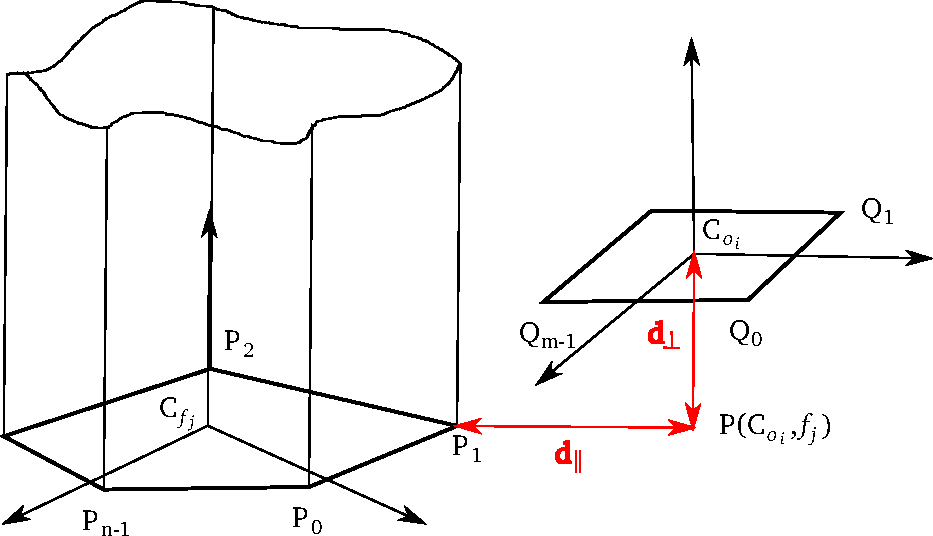
\includegraphics[width=\linewidth]{figures/convex-shape-contact.pdf}
  \end{center}
  \caption{Distance defined by two convex polygons.}
  \label{fig:convex-shape-contact}
\end{figure}

When an object is not grasped, it should lie in a stable pose. There are two simple methods to enforce that:
\begin{enumerate}
\item defining virtual grippers in the environment and virtual handles on the object, implicitly defines a discrete set of poses,
\item defining a virtual gripper on an horizontal plane and a virtual handle on the object, and using a grasp with flags $(\false,\false,\true,\true,\true,\false)$ constrains the object to move on a infinite horizontal plane.
\end{enumerate}

Here we propose a third method that enables users to define contact surfaces in a more flexible way. In this aim, we denote by:
\begin{itemize}
\item $(o_i)_{i\in I}$ a set of convex polygons attached to an object,
\item $(f_j)_{j\in J}$ a set of convex polygons attached to the environment or to a mobile part of a robot that can receive objects (mobile robot for example),
\item respectively $C_{o_i}$, $\mathbf{n}_{o_i}$ the barycenter of $o_i$ and the normal to the plane containing $o_i$,
\item $C_{f_j}$, $\mathbf{n}_{f_j}$ the barycenter of $f_j$ and the normal to the plane containing $f_j$,
\item $P(C_{o_i},f_j)$, the orthogonal projection of $C_{o_i}$ onto the plane containing $f_j$.
\end{itemize}
Then we define the distance between polygons $o_i$ and $f_j$ as the distance of $C_{o_i}$ to the cylindrical volume of generatrix $\mathbf{n}_{f_j}$ and of directrix $f_j$:
\begin{align}\label{eq:contact-distance}
  d(f_j,o_i) = \sqrt{d_{\parallel}^2 + d_{\perp}^2}
\end{align}
where
\begin{align*}
  i,j & \mbox{ are the indices that minimize the above distance,}\\
d_{\parallel} &= \left\{\begin{array}{lll} d(f_j,P(C_{o_i},f_j))&\mbox{if}& P(C_{o_i},f_j)\mbox{ outside } f_j\\
0 & & \mbox{otherwise}
\end{array}\right. \\
d_{\perp} &= \mathbf{n}_{f_j}.\vec{C_{f_j}C_{o_i}}.
\end{align*}
Figure~\ref{fig:convex-shape-contact} illustrates this definition.

We denote by $o_i(\conf)$ and $f_j(\conf)$ the poses in configuration $\conf$ of frames with respective centers $C_{o_i}$ and $C_{f_j}$ and with $x$-axis normal to each polygon. In an analogous way as in Definition~\ref{def:grasp}, we define
\begin{equation}\label{eq:convex-shape-contact-hbar}
\bar{h}(\conf) = \log_{\reals^3\times SO(3)} \left(f_{j}(\conf)^{-1}o_i(\conf)\right)
\end{equation}
The contact constraint is defined by the following piece-wise differentiable function:
\begin{equation}\label{eq:convex-shape-contact}
h(\conf) = \left\{\begin{array}{lll}(\bar{h}_1,0,0,\bar{h}_5,\bar{h}_6)&
\mbox{if} & P(C_{o_i},f_j)\mbox{ inside } f_j\\
(\bar{h}_1,\bar{h}_2,\bar{h}_3,\bar{h}_5,\bar{h}_6)&
\mbox{if} & P(C_{o_i},f_j)\mbox{ outside } f_j\end{array}\right.
\end{equation}
It is straightforward that the above function vanishes if and only if two convex polygons $o_i$ and $f_j$ are in contact and $C_{o_i}$ is inside $f_j$.

As for grasps, we need to define a parameterized complement constraint for the contact constraint in order to specify the sub-manifold of configurations that are reachable from one configuration while keeping the object in a constant stable pose. The naive way consists in defining
$$
h_{comp}(\conf) = \left\{\begin{array}{lll}(\bar{h}_2,\bar{h}_3,\bar{h}_4)&
\mbox{if} & P(C_{o_i},f_j)\mbox{ inside } f_j\\
(0,0,\bar{h}_4)&
\mbox{if} & P(C_{o_i},f_j)\mbox{ outside } f_j\end{array}\right.
$$
$\bar{h}_2$, $\bar{h}_3$, $\bar{h}_4$ respectively represent the translation in $y-z$ plane and the rotation around $x$-axis of frame $o_i$ with respect to frame $f_j$. Let $\conf_0$ be a configuration such that $h(\conf_0)=0$. The sub-manifold defined by
\begin{equation}\label{eq:stable-pose}
\left\{\conf\in\CS,\ \ h(\conf)=0\ \ h_{comp}(\conf) = h_{comp}(\conf_0) \right\}
\end{equation}
contains one object pose for each pair of polygons $(o_i,f_j)$, and there are
$|I| . |J|$ possible combinations. Thus this constraint is not suitable to
enforce object immobility along a path since the object may jump from one pose to another one.

To disambiguate the various combinations of convex polygons that can be in contact, we define
\begin{equation}\label{eq:convex-shape-contact-complement}
h_{comp}(\conf) = \left\{\begin{array}{l}(\bar{h}_2 + 2jM,\bar{h}_3 + 2iM,\bar{h}_4)\\
\mbox{if } P(C_{o_i},f_j)\mbox{ inside } f_j\\
(2jM,2iM,\bar{h}_4)\\
\mbox{if } P(C_{o_i},f_j)\mbox{ outside } f_j\end{array}\right.
\end{equation}
where
\begin{itemize}
\item $i$ and $j$ are the indices that minimize distance~(\ref{eq:contact-distance}),
\item $M$ is a positive real number such that for any $\kappa\in J$, all vertices of $f_\kappa$ are included in the disk of center $C_{f_\kappa}$ and of radius $M$.
\end{itemize}
With this definition, the sub-manifold defined by~(\ref{eq:stable-pose}), (\ref{eq:convex-shape-contact}), (\ref{eq:convex-shape-contact-complement}) contains configurations where the object is in a unique stable pose. The polygon indices $i$ and $j$, as well as their relative position can indeed be recovered from~(\ref{eq:convex-shape-contact-complement}):
\begin{align*}
  i &= \left\lfloor\frac{\bar{h}_3}{2M} + \frac{1}{2}\right\rfloor\\
  j &= \left\lfloor\frac{\bar{h}_2}{2M} + \frac{1}{2}\right\rfloor\\
  \bar{h}_1 &= \bar{h}_5 = \bar{h}_6 = 0\\
  \bar{h}_2 &= h_{comp\ 1} - 2jM\\
  \bar{h}_3 &= h_{comp\ 2} - 2iM\\
  \bar{h}_4 &= h_{comp\ 3}
\end{align*}
and from (\ref{eq:convex-shape-contact-hbar}),
$$
f_{j}(\conf)^{-1}o_i(\conf) = \exp_{\reals^3\times SO(3)}\left(\bar{h}\right).
$$
Uniqueness comes from the fact that when two convex polygons are in contact,
necessarily, $|\bar{h}_2| \leq M$,$|\bar{h}_3| \leq M$.
% Remark about convergence of the solver and about explicit constraint.

\subsection{Merging constraint and complement into an explicit constraint}
\label{subsec:explicit}

Note that when a grasp constraint and its complement are combined, they
constitute an explicit constraint since the pose of the object grasped
uniquely depends on the configuration of the robot that grasps the object.

Similarly, when a placement constraint and its complement are combined, they
constitute an explicit constraint since the pose of the object placed uniquely
depends on the pose of the contact surface on which the object is placed. This
latter pose
\begin{itemize}
\item either depends on the configuration of the robot the contact surface
  belongs to,
\item or is constant if the contact surface belongs to the environment.
\end{itemize}
In any case, the explicit expression of the object pose depends on the right
hand side of the complement constraint that is constant along transition paths.

During the construction of the constraint graph (described in Section~\ref{subsec:constraint graph}), grasp and placement
constraints, their complements and the associated explicit constraints
are created together and registered using method\\
\texttt{registerConstraint} of Class
\href{https://gepettoweb.laas.fr/hpp/hpp-manipulation/doxygen-html/classhpp_1_1manipulation_1_1graph_1_1Graph.html}{\texttt{ConstraintGraph}}.

\subsection{Constraint Graph}\label{subsec:constraint graph}

According to Definition~\ref{def:manipulation-problem}, the set of admissible configurations of a manipulation problem is the union of sub-manifolds of the configuration space of the system. Each sub-manifold is defined by grasp and/or stable contact constraints. We call each sub-manifold a \textit{state} of the problem.

A state can be defined by a subset of active grasps, any object not grasped being in a stable contact pose. Let $\ngrippers$, $\nhandles$, and $\nobjects$ respectively denote the number of grippers, handles, and objects.

We denote by
\begin{itemize}
\item $grasp_{ij}\ i\in\{1,\cdots,\ngrippers\}\ j\in\{1,\cdots,\nhandles\}$ the grasp constraint of handle $j$ by gripper $i$,
\item $grasp_{ij}/comp\ i\in\{1,\cdots,\ngrippers\}\ j\in\{1,\cdots,\nhandles\}$ the complement constraint of the latter,
\item $place_{i}\ i\in\{1,\cdots\nobjects\}$ the placement constraint of object $i$,
\item $place_{i}/comp\ i\in\{1,\cdots\nobjects\}$ the complement constraint of the latter.
\end{itemize}


A state $\state$ is denoted by a vector of size $\ngrippers$:
\begin{equation}\label{eq:state}
\state = \left(h_1,\cdots,h_{\ngrippers}\right)
\end{equation}
where $h_i\in\{\emptyset,1,\cdots,\nhandles\}$ denotes the index of the handle grasped by gripper $i$; $h_i=\emptyset$ means that gripper $i$ does not grasp any handle.

\paragraph{Number of states} note that for $i\in\{1,\cdots,\nhandles\}$ the number of occurrences of $i$ in $\state$ is at the most 1: a handle cannot be grasped by several grippers. Note also that the number of occurrences of $\emptyset$ is not limited: several grippers may hold nothing. Let $m$ be a non-negative integer not greater than $\ngrippers$ nor $\nhandles$ and let us count the number of states with $m$ handles grasped. The number of subset of $m$ handles among $\nhandles$ is equal to $\frac{\nhandles!}{(\nhandles-m)!m!}$. And the number of ways of dispatching them among the $\ngrippers$ grippers is equal to $\frac{\ngrippers!}{(\ngrippers-m)!}$. Thus, the total number of states is equal to
$$
\sum_{m=0}^{\min(\ngrippers,\nhandles)} \frac{\nhandles!}{(\nhandles-m)!m!} \frac{\ngrippers!}{(\ngrippers-m)!}
$$
\begin{definition}\label{def:neighboring-states}\textbf{Neighboring states}\\
  Two states $\state_1=(h_{1 1},\cdots,h_{\ngrippers 1})$ and $\state_2=(h_{1 2},\cdots,h_{\ngrippers 2})$ are neighboring if they differ by only one grasp and the grasp is empty in one of the states:
  \begin{align*}
    &\exists i\in\{1,\cdots,\ngrippers\},\,h_{i 1} \not= h_{i 2} \mbox{ and } (h_{i 1}=\emptyset \mbox{ or } h_{i 2}=\emptyset), \mbox{ and }\\
    &\forall j\in\{1,\cdots,\ngrippers\},\, j\not=i,h_{j 1} = h_{j 2}.
  \end{align*}
\end{definition}
\begin{definition}\label{def:constraint-graph}\textbf{Constraint graph}\\
  The constraint graph related to a manipulation problem as defined in Definition~\ref{def:manipulation-problem} is a graph
  \begin{itemize}
  \item the nodes of which are states defined by subsets of grasps~(\ref{eq:state}),
  \item two edges (back and forth) connect two states if they are neighboring,
  \item one edge connects each state to itself.
  \end{itemize}
  Edges are also called \textit{transitions}.
  Nodes contain
  \begin{itemize}
  \item the grasp constraints that are active in the corresponding state,
  \item a placement constraint for each object that is not grasped by any handle.
  \end{itemize}
  Transitions contain
  \begin{itemize}
  \item the constraints of the node they connect with the least active grasps,
  \item the parameterized complement constraint of each of the latter.
  \end{itemize}
\end{definition}

\subsection{Example}\label{subsec:ur3-cylinder}

To illustrate the notions expounded in the previous sections, let us consider an example of two UR3 robots manipulating a cylinder illustrated in Figure~\ref{fig:2ur3-cylinder}. The robot is fitted with one gripper attached to the end-effector. The cylinder is equipped with two handles and with two square contact surfaces corresponding to the top and bottom faces of the cylinder. $\ngrippers=2,\nhandles=2,\nobjects=1$. The flag of the handles are
$$(\true,\true,\true,\false,\true,\true).$$
Therefore grasp constraints are of dimension 5 and keep the rotation of the gripper around the cylinder axis free.
\begin{table}
  \begin{center}
    \begin{tabular}{|p{.44\linewidth}|p{.44\linewidth}|}
      \hline
      state & active constraints\\
      \hline
      $(\emptyset,\emptyset)$ & $place_1$ \\
      $(j,\emptyset),\,j\in\{1,2\}$ & $grasp_{1j}$\\
      $(\emptyset,j),\,j\in\{1,2\}$ & $grasp_{2j}$\\
      $(i,j)\,i,j\in\{1,2\}$ & $grasp_{1i},grasp_{2j}$\\
      \hline
    \end{tabular}
  \end{center}
  \caption{State constraints.}
  \label{tab:state-constraints}
\end{table}
Table~\ref{tab:state-constraints} indicates which constraints are active for each state. Table~\ref{tab:transition-constraints} indicates which constraints are active for each transition.

\begin{table}
  \begin{center}
    \begin{tabular}{|p{.25\linewidth}|p{.18\linewidth}|p{.41\linewidth}|}
      \hline
      transition & belongs to & additional constraints\\
      \hline
      $(\emptyset,\emptyset)\rightarrow (i,\emptyset)$ & $(\emptyset,\emptyset)$ & $place_1/comp$\\
      $(\emptyset,\emptyset)\rightarrow (\emptyset,i)$ & $(\emptyset,\emptyset)$ & $place_1/comp$\\
      $(i,\emptyset)\rightarrow(i,j)$ & $(i,\emptyset)$ & $grasp_{1i}/comp$\\
      $(\emptyset,j)\rightarrow(i,j)$ & $(\emptyset,j)$ & $grasp_{2j}/comp$\\
      \hline
    \end{tabular}
  \end{center}
  \caption{Transition constraints: $i,j$ are either 1 or 2. column
    "belongs to" means that paths along the transition belong to the
    state, \textit{i.e.} the transition contains the state
    constraints.}
  \label{tab:transition-constraints}
\end{table}

\subsection{Automatic construction}

\begin{algorithm}
  \algblockdefx[globalVariable]{GlobalVariable}{EndGlobalVariable}{\textbf{global variables}}{}
  \begin{algorithmic}[1]
    \GlobalVariable
    \State{$\nobjects$}\Comment{number of objects}
    \State{$\ngrippers$}\Comment{number of grippers}
    \State{$\nhandles$}\Comment{number of handles}
    \EndGlobalVariable
    \Function{buildConstraintGraph}{}
    \State{$\mathcal{G}\gets\left[0,\cdots,\ngrippers-1\right]$}
    \Comment{list of gripper indices}
    \State{$\mathcal{H}\gets\left[0,\cdots,\nhandles-1\right]$}
    \Comment{list of handle indices}
    \State {$Gr\gets\left[\emptyset,\cdots,\emptyset\right]$}\Comment{list of size $\ngrippers$}
    \State \Call{recurse}{$\mathcal{G}$,$\mathcal{H}$,$Gr$}
    \EndFunction
    \Function{recurse}{$\mathcal{G}$,$\mathcal{H}$,$Gr$}
    \State\Call{createState}{$Gr$}
    \If{$\mathcal{G}=\emptyset$ or $\mathcal{H}=\emptyset$}
    \State{\Return}
    \EndIf
    \For{$g$ in $\mathcal{G}$}
    \State{$\mathcal{G}^{\prime}\gets \mathcal{G}\setminus\{g\}$}
    \For{$h$ in $\mathcal{H}$}
    \State{$\mathcal{H}^{\prime}\gets\mathcal{H}\setminus\{h\}$}
    \State{$Gr^{\prime}\gets Gr$}
    \State{$Gr^{\prime}[g]\gets h$}
    \State{$isNewState\gets\mathbf{not}\ $\Call{existState}{$Gr^{\prime}$}}
    \State{\Call{createState}{$Gr^{\prime}$}}
    \State{\Call{createTransition}{$Gr$, $Gr^{\prime}$}}
    \If{$isNewState$}{\ \Call{recurse}{$\mathcal{G}^{\prime}$,$\mathcal{H}^{\prime}$,$Gr^{\prime}$}}\label{cond:recurse}
    \EndIf
    \EndFor
    \EndFor
    \EndFunction
  \end{algorithmic}
  \caption{Recursive Construction of the constraint graph. The
    construction starts by the state with no grasp. Call to
    {\scriptsize RECURSE} function loops over the available grippers
    and handles and creates states with one more grasp, and a
    transition to these new states. In each state, a placement
    constraint is added for each object of which no handle is
    grasped. Variables $\mathcal{G}$ and $\mathcal{H}$ contain the
    indices of the free grippers and handles. Variable $Gr$ stores the
    current set of grasps following Expression~(\ref{eq:state}).
    Lines~\ref{beg:comp-placement-constraints} to
    \ref{end:comp-placement-constraints}
    compute which objects are not grasped.
    Lines~\ref{beg:set-placement-constraints} to
    \ref{end:set-placement-constraints} insert placement constraints in the
    state for those objects. Line~\ref{cond:recurse} recurses only if the
    latest node reached is new. Functions \CREATESTATE and \CREATETRANSITION are given in Algorithm~\ref{algo:createStateAndTransition}.}
  \label{algo:constraintGraphFactory}
\end{algorithm}
\begin{algorithm}
  \begin{algorithmic}[1]
    \Function{createState}{$Gr$}
    \If{\Call{existState}{$Gr$}}\State{\Return}\EndIf
    \State{$\state\gets\mbox{ new state}$}
    \State{$\state.Pl\gets\left[\true,...,\true\right]$}\Comment{list of size $\nobjects$}\label{beg:comp-placement-constraints}
    \For{$g\mbox{ in } \left[0,\cdots,\ngrippers-1\right]$}
    \State{$h\gets Gr[g]$}
    \State{$\state.Pl[\Call{objectIndex}{h}]\gets\false$}
    \State{$\state$.\ADD(\Call{graspConstraint}{g,h})}
    \EndFor\label{end:comp-placement-constraints}
    \For{$o\mbox{ in }\left[0,\cdots,\nobjects\right]$}
    \If{$\state.Pl[o]$}
    \State{$\state$.\ADD(\Call{placeConstraint}{$o$}})
    \EndIf
    \EndFor
    \EndFunction
    \Function{createTransition}{$Gr_1,Gr_2$}
    \State{$\transition\gets\mbox{ new transition}(Gr_1,Gr_2)$}
    \State{$\state_1\gets$\Call{state}{$Gr_1$}}\Comment{Recover state for this set of grasps}
    \For{$g\mbox{ in } \left[0,\cdots,\ngrippers-1\right]$}
    \State{$h\gets Gr_1[g]$}
    \State{$\transition$.\ADD(\Call{graspConstraint}{g,h})}
    \State{$\transition$.\ADD(\Call{graspConstraintComp}{g,h})}
    \EndFor
    \For{$o\mbox{ in }\left[0,\cdots,\nobjects\right]$}
    \label{beg:set-placement-constraints}
    \If{$\state_1.Pl[o]$}
    \State{$\transition$.\ADD(\Call{placeConstraint}{$o$}})
    \State{$\transition$.\ADD(\Call{placeConstraintComp}{$o$}})
    \EndIf
    \EndFor\label{end:set-placement-constraints}
    \State{$\transition_1 \gets\mbox{ new transition}(Gr_2,Gr_1)$}
    \State{$\transition_1$.\SETCONSTRAINTS(\Call{$\transition$.{\scriptsize CONSTRAINTS}})}
    \EndFunction
  \end{algorithmic}
  \caption{Method \CREATESTATE builds the constraints relative to a state: one grasp constraint for each grasp, and one placement constraint for each object non grasped. \CREATETRANSITION builds the constraints relative to a transition: the constraints of the initial state (with the fewest grasps) and their complements.}
  \label{algo:createStateAndTransition}
\end{algorithm}

Given a set of grippers, handles and objects, the constraint graph can be constructed automatically. \href{https://github.com/humanoid-path-planner/hpp-manipulation-corba/blob/5af1b3bad68e8c339d5f42eb72173d7356504532/src/hpp/corbaserver/manipulation/constraint_graph_factory.py\#L187}{Here} is an implementation in python. Algorithm~\ref{algo:constraintGraphFactory} describes this implementation.
Functions
\begin{itemize}
\item {\scriptsize GRASP}{\small C}{\scriptsize ONSTRAINT},
\item {\scriptsize GRASP}{\small C}{\scriptsize ONSTRAINT}{\small C}{\scriptsize OMP}, build grasp constraint and complement constraint as defined in Section~\ref{subsec:grasp},
\item {\scriptsize PLACE}{\small C}{\scriptsize ONSTRAINT},
\item {\scriptsize PLACE}{\small C}{\scriptsize ONSTRAINT}{\small C}{\scriptsize OMP} build placement constraints and complement as defined in Section~\ref{subsec:placement},
\item {\scriptsize EXIST}{\small S}{\scriptsize TATE}($Gr$) returns $\true$ if a state has already been created for the set of grasps given as input,
\item{\scriptsize STATE}($Gr$) returns the state created with the set of grasps given as input,
\item {\scriptsize OBJECT}{\small I}{\scriptsize NDEX}($h$) returns the index of the object handle $h$ belongs to.
\end{itemize}

\section{Manipulation planning}\label{sec:manipulation-planning}

In this section, we show how the constraint graph defined in the previous section is used to plan collision-free manipulation paths. Although we are working on an extension of the RMR* algorithm~\cite{schmitt17icra} to several grippers, objects and handles, the only manipulation planning algorithm available up to now in HPP is an extension of the RRT algorithm described in the next section.

\subsection{Manipulation-RRT}

Manipulation Randomly exploring Random Tree is an extension of the RRT algorithm~\cite{LavKuf01b} that grows trees in the free configuration space, exploring the different states of the manipulation problem. Algorithm~\ref{algo:M-RRT} describes the algorithm implemented in C++ \href{https://github.com/humanoid-path-planner/hpp-manipulation/blob/16369aa291ab1b17ef6176ae8b8b2512b5e6fff7/src/manipulation-planner.cc\#L159}{here}.

After initializing the roadmap with the initial and goal configurations, the algorithm iteratively calls method {\scriptsize ONE}{\small S}{\scriptsize TEP} until a solution path is found or the maximum number of iterations is reached.
This latter method shoots a random configuration (line 6) and for each connected component of the roadmap and each state of the constraint graph, extends the nearest node in the direction of the random configuration (lines 7--10). For each successful extension, the end of the extension path is stored for later connection (line 11). After the extension step, the algorithm tries to connect new nodes to other connected components using two strategies:
\begin{enumerate}
\item function \TRYCONNECTNEWNODES calls method \CONNECT between all pairs of new nodes,
\item function \TRYCONNECTTOROADMAP tries to connect each new node to the nearest nodes in other connected components of the roadmap also using function \CONNECT.
\end{enumerate}
Function \CONNECT attempts to connect two configurations in two states. First, it checks whether there exists a transition between the states. If so, it checks that the right hand side of the transition parameterized constraints is the same for both configurations (up to the error threshold). Then it returns the linear interpolation between the configurations, projected onto the sub-manifold defined by the transition constraints. If the path is in collision {\color{blue}or discontinuous}, only the {\color{blue}continuous} collision-free part at the beginning of the path is returned.

Function \EXTEND attempts to generate a path from a configuration in a state to another state following a random transition. Similarly as for function \CONNECT, the path is projected onto the sub-manifold defined by the transition constraints. The end configuration is obtained by applying to the random configuration the constraints of the transition and of the goal state.
\begin{algorithm}
  \begin{algorithmic}[1]
    \Function{initializeRoadmap}{$\conf_{init}$,$\conf_{goal}$}
    \State$\roadmap\gets\mbox{ new roadmap}$
    \State{$\roadmap$.\Call{addNode}{$\conf_{init}$};
      $\roadmap$.\Call{addNode}{$\conf_{goal}$}}
    \EndFunction
    \Function{oneStep}{$\roadmap$}
    \State{$newNodes\gets$ empty list}
    \State{$\conf_{rand}\gets$\Call{shootRandomConfig}{ }}
    \For{$cc$ in connected components of $\roadmap$}
    \For{$s$ in constraint graph states}
    \State{$\conf_{near}\gets$\Call{nearestNode}{$cc$,$s$,$\conf_{rand}$}}
    \State{$p\gets$\Call{extend}{$s$, $\conf_{near}$, $\conf_{rand}$}}
    \If{$p$}$\,newNodes\gets\,newNodes\cup\{\mbox{end of}\,p\}$\EndIf
    \EndFor
    \EndFor
    \State{$nc\gets$\Call{tryConnectNewNodes}{$\roadmap$, $newNodes$}}
    \If{$nc=0$}
    \State{\Call{tryConnectToRoadmap}{$\roadmap$,$newNodes$}}
    \EndIf
    \EndFunction
    \Function{tryConnectNewNodes}{$\roadmap$, $nodes$}
    \For{$\conf_1,\conf_2\mbox{ in } nodes,\ \conf_1\not=\conf_2$}
    \State{$s_1\gets\Call{state}{\conf_1};s_2\gets\Call{state}{\conf_2}$}
    \State{$p\gets\Call{Connect}{\conf_1,s_1,\conf_2,s_2}$}
    \If{$p$}
    \State{$\roadmap$.\Call{addEdge}{$\conf_1$,$\conf_2$,$p$}}
    \EndIf
    \EndFor
    \EndFunction
    \Function{tryConnectToRoadmap}{$\roadmap$,$nodes$}
    \For{$\conf_1\mbox{ in } nodes$}
    \State{$s_1\gets\Call{state}{\conf_1}$}
    \For{$cc$ in connected components of $\roadmap$}
    \If{$\conf_1\notin cc$}
    \State{$near\gets K\mbox{ nearest neighbors of }\conf_1\mbox{ in }cc$}
    \For{$\conf_2\mbox{ in }near$}
    \State{$s_2\gets\Call{state}{\conf_2}$}
    \State{$p\gets\Call{Connect}{\conf_1,s_1,\conf_2,s_2}$}
    \If{$p$}{$\roadmap$.\Call{addEdge}{$\conf_1,\conf_2$}}\EndIf
    \EndFor
    \EndIf
    \EndFor
    \EndFor
    \EndFunction
    \Function{extend}{$s$, $\conf_{near}$, $\conf_{rand}$}
    \State{$solver\gets$\Call{SolverBySubstitution}{}}
    \State{$\transition\gets$ random edge getting out of $s$}
    \State{$g\gets$ state $\transition$ points to}
    \For{$c$ in $g$.\Call{constraints}{ }}
    \State{$solver$.\Call{addConstraint}{$c(\conf)=0$}}
    \EndFor
    \For{$c$ in $\transition$.\Call{constraints}{ }}
    \State{$solver$.\Call{addConstraint}{$c(\conf) = c(\conf_{near})$}}
    \EndFor
    \State{$\conf_{target}\gets solver$.\Call{solve}{$\conf_{rand}$}}
    \If{$\conf_{target}$}
    \State{$p\gets$ linear interpolation from $\conf_{near}$ to $\conf_{target}$}
    \State{$p$.\Call{addConstraints}{$\transition$.{\scriptsize CONSTRAINTS}()}}
    \EndIf
    \If {$p$ collision-free \color{blue}and continuous} {\Return $p$}
    \Else { \Return collision-free {\color{blue}continuous} portion of $p$ starting at $\conf_{near}$}
    \EndIf
    \EndFunction
  \end{algorithmic}
  \caption{Manipulation RRT algorithm iteratively calls method {\scriptsize ONE}{\small S}{\scriptsize TEP} until a solution path is found or the maximum number of iterations is reached. Function \CONNECT is described in Algorithm~\ref{algo:M-RRT-connect}}
  \label{algo:M-RRT}
\end{algorithm}
\begin{algorithm}
  \begin{algorithmic}
    \Function{connect}{$\conf_1,s_1,\conf_2,s_2$}
    \State{parameter $\epsilon>0$}
    \State{$p\gets$ linear interpolation from $\conf_1$ to $\conf_2$}
    \State{$\transition\gets$\Call{transition}{$s_1$,$s_2$}}
    \If{not $\transition$}{ \Return $\emptyset$}
    \EndIf
    \For{$c$ in $\transition$.\Call{constraints}{ }}
    \If{$\|c(\conf_2) - c(\conf_1)\|\geq\epsilon$}{ \Return $\emptyset$}
    \Else
    \State{$p$.\Call{addConstraint}{$c(\conf)=c(\conf_1)$}}
    \EndIf
    \EndFor
    \If {$p$ in collision} { \Return $\emptyset$}
    \EndIf
    \State{\Return $p$}
    \EndFunction
  \end{algorithmic}
  \caption{Function \CONNECT of M-RRT algorithm}
  \label{algo:M-RRT-connect}
\end{algorithm}

\subsection{Examples}

\begin{figure}
  \begin{center}
    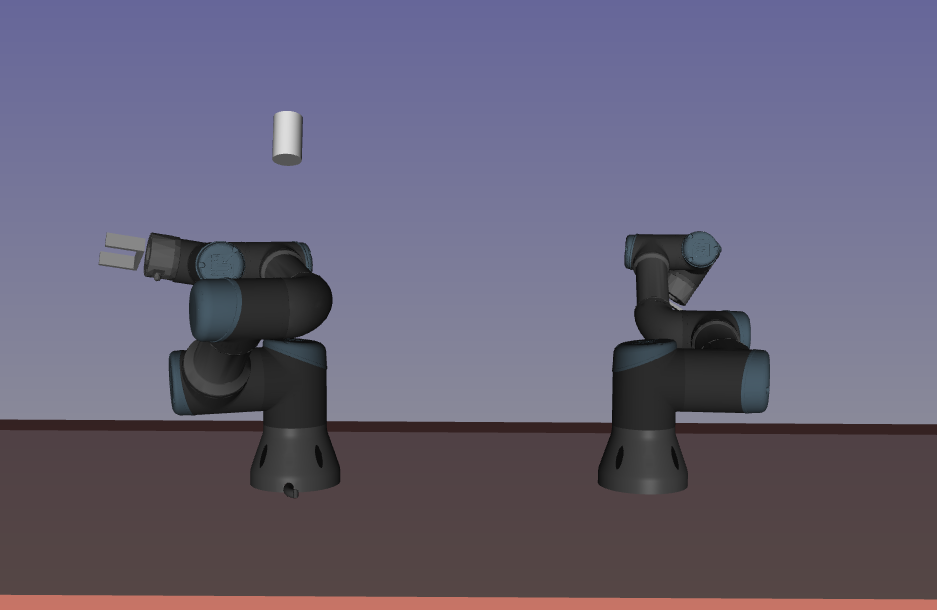
\includegraphics[width=\linewidth]{figures/example-qrand-2.png}
    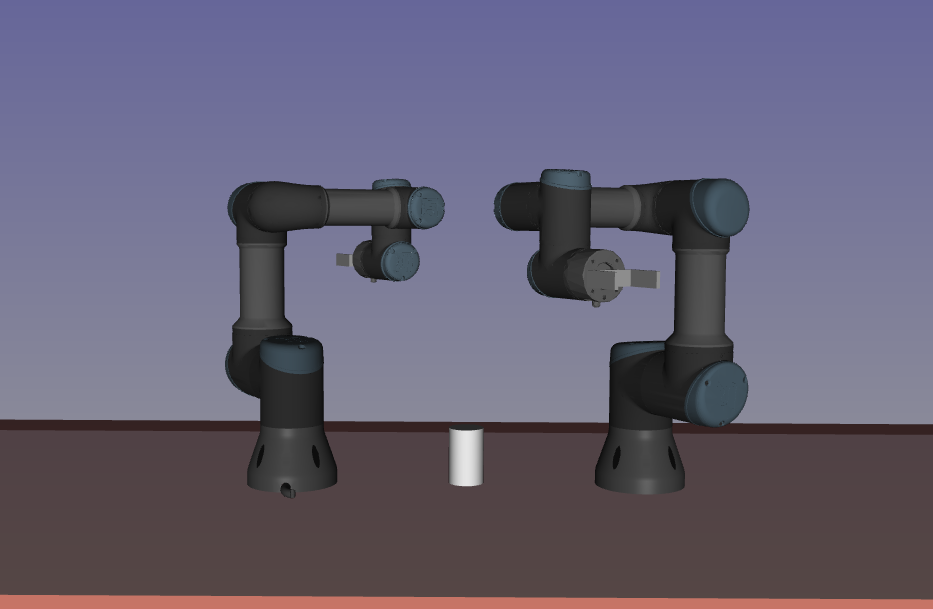
\includegraphics[width=\linewidth]{figures/example-q0-2.png}
    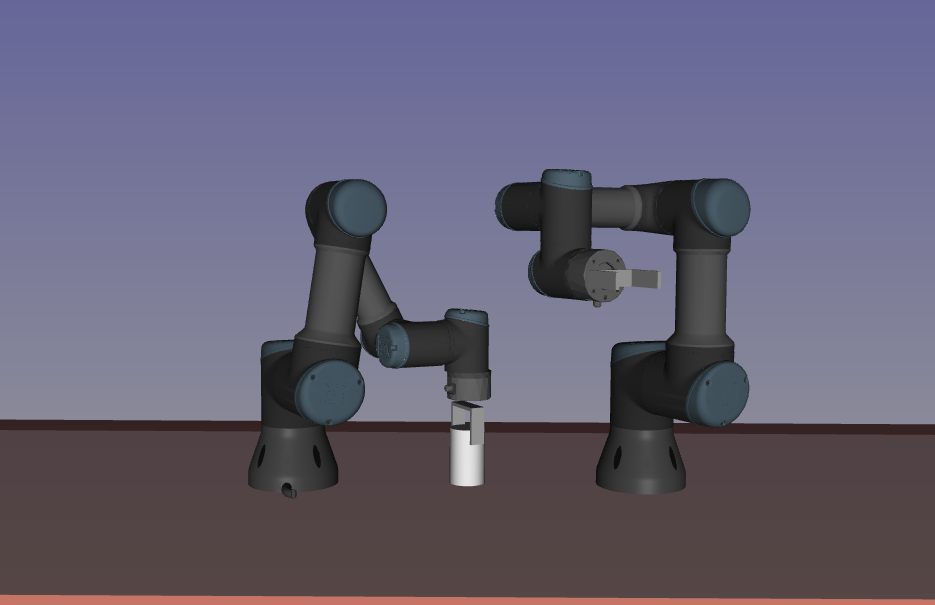
\includegraphics[width=\linewidth]{figures/example-q-wp-2.png}
  \end{center}
  \caption{Example of extension along a transition of the constraint graph. Top
    $\conf_{rand}$, middle $\conf_{near}$, bottom $\conf_{target}$.
  }
  \label{fig:MRRT-extension}
\end{figure}

In this section, we illustrate the algorithm described in the previous section with two examples. Figure~\ref{fig:MRRT-extension} illustrates function \EXTEND defined in the previous section on the example of Figure~\ref{fig:2ur3-cylinder}.
The system considered is
composed of two robots and a cylinder with two handles. The top picture displays
$\conf_{rand}$. The middle picture displays $\conf_{near}$ that belongs to state
$(\emptyset,\emptyset)$. The transition that is randomly selected
(Algorithm~\ref{algo:M-RRT}, line 33) is
$(\emptyset,\emptyset) \rightarrow (1,\emptyset)$, meaning that robot 1 will
try to grasp handle 1. According to tables~\ref{tab:state-constraints} and
\ref{tab:transition-constraints}, the constraints of the transition are
$(place_1, place_1/comp)$.
The first one is of type~(\ref{eq:convex-shape-contact}), the second one is
of type~(\ref{eq:convex-shape-contact-complement}) and is parameterized: the
right hand side uniquely defines the contact surfaces and the position of the
object on the contact surface. $\conf_{target}$ is obtained by projecting $\conf_{rand}$
onto the manifold defined by the following constraints
(Algorithm~\ref{algo:M-RRT}, lines 35--39):
\begin{itemize}
\item $place_1$, $place_1/comp$ that belong to the transition,
\item $grasp_{11}$ that belongs to the goal state.
\end{itemize}
According to Section~\ref{subsec:explicit}, the first two constraints can be
replaced by an explicit constraint: the position of the object can be deduced
from the right hand side of $place_1/comp$ that is initialized with configuration
$\conf_{near}$.

After substitution, the set of constraints is reduced to an implicit constraint
on the configuration variables of robot 1 (6 variables). The solution found by the solver, $\conf_{target}$ (line 39) is displayed in
Figure~\ref{fig:MRRT-extension} bottom. Notice that as expected, the position of the object is the same in $\conf_{target}$ as in $\conf_{near}$.

The path returned by function \EXTEND is the linear interpolation between
$\conf_{near}$ and $\conf_{target}$ constrained with $place_1$, $place_1/comp$ with
right hand side initialized with $\conf_{near}$. As explained earlier, this
constraint is replaced by an explicit constraint. Let us notice that the linear interpolation already satisfies the constraint, but this is not always the case.

If the latter path is in collision, the collision-free part of the path starting
at $\conf_{near}$ is returned.

\begin{figure}
  \begin{center}
    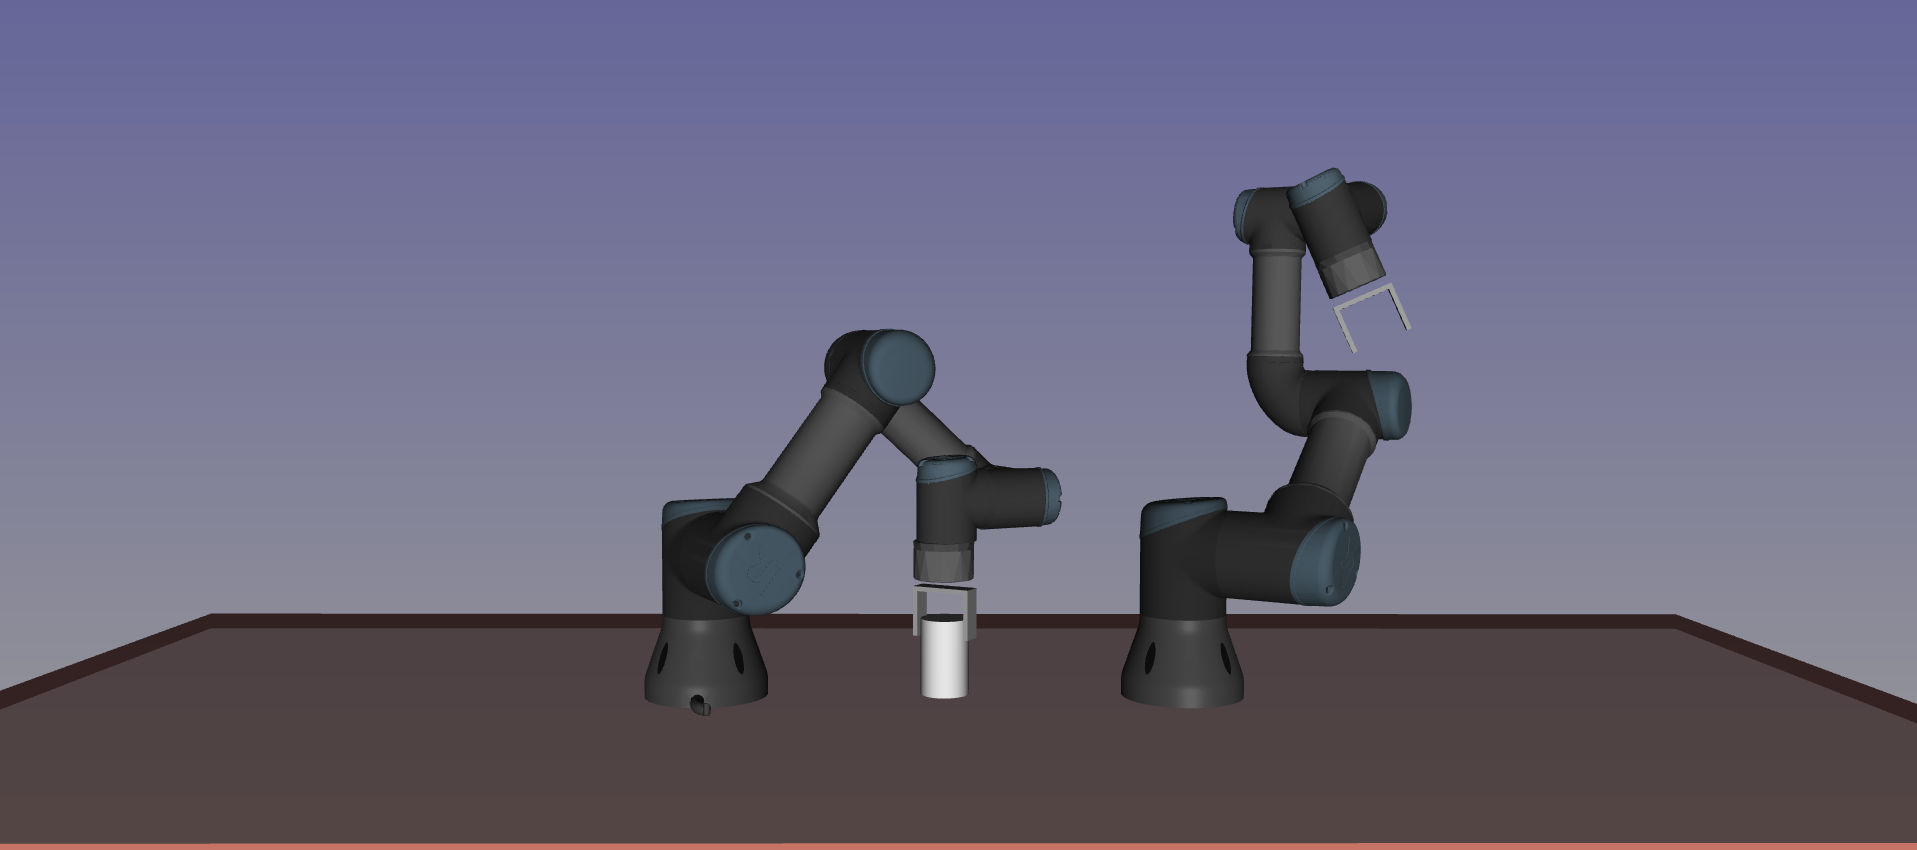
\includegraphics[width=.75\linewidth]{figures/example-qtarget-1.png}
    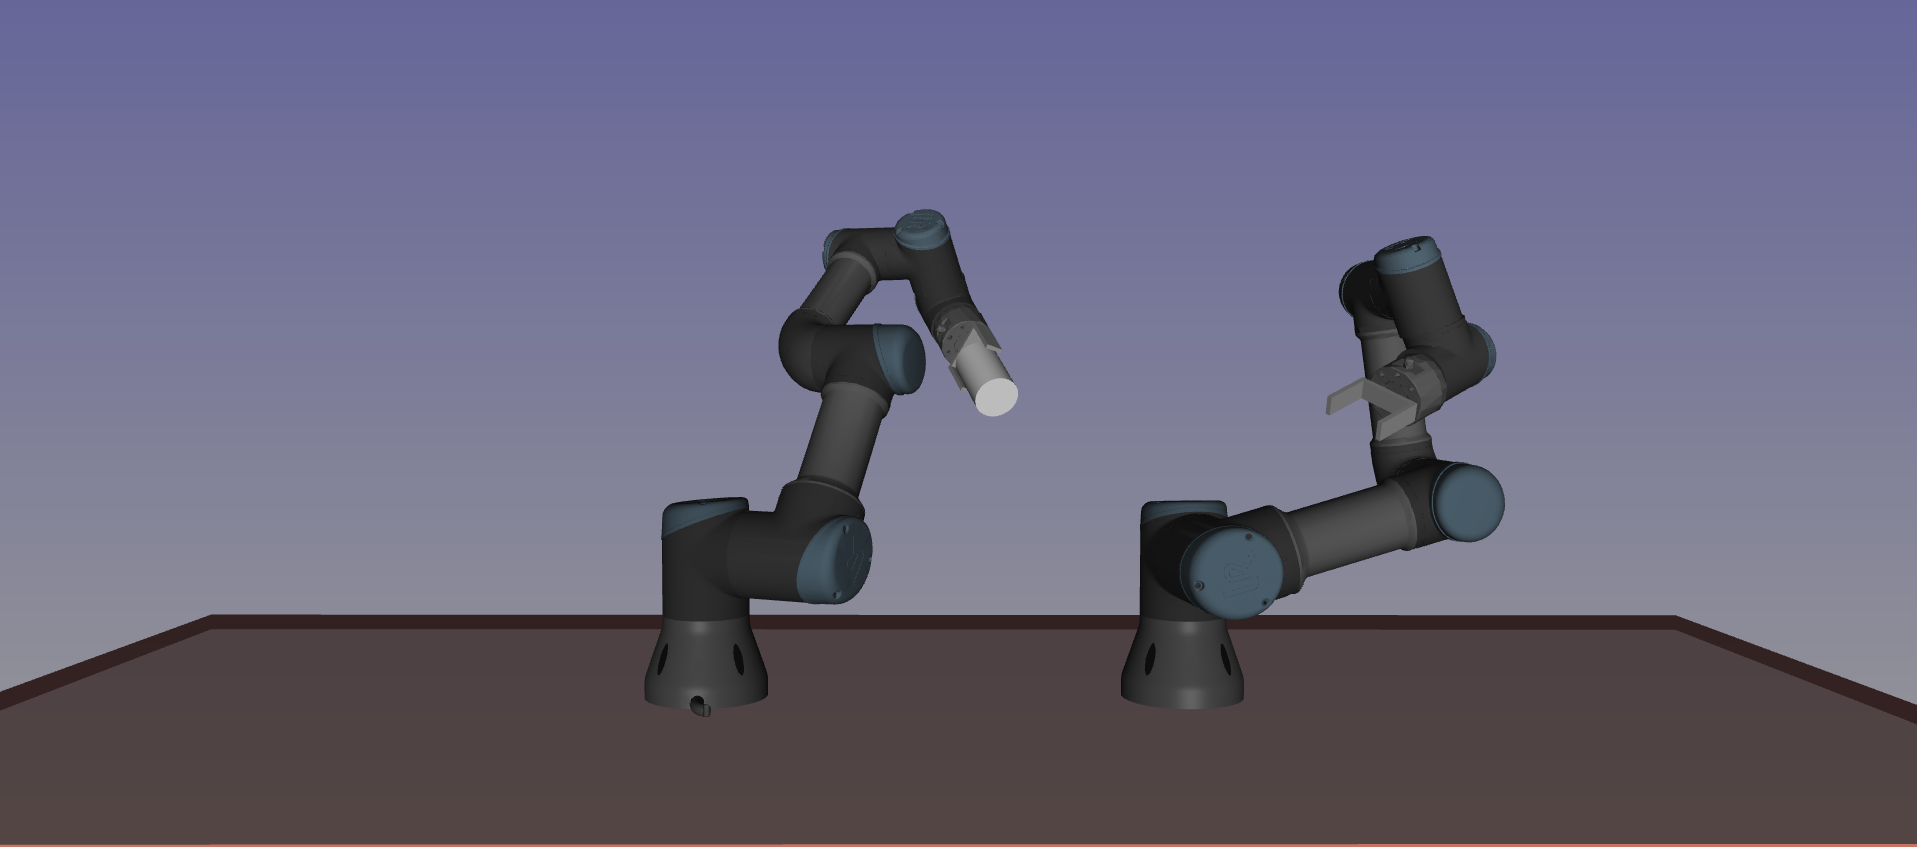
\includegraphics[width=.75\linewidth]{figures/example-connect-q1.png}
  \end{center}
  \caption{Method \CONNECT applied to two configurations.}
  \label{fig:connect}
\end{figure}

Figure~\ref{fig:connect} illustrates method \CONNECT applied to two configurations $\conf_1$ (top) and $\conf_2$ (bottom). Both configurations belong to state $(1,\emptyset)$\footnote{Note that $\conf_1$ is at the intersection between states
  $(\emptyset,\emptyset)$ and $(1,\emptyset)$.}. The transition between those states $(1,\emptyset)\rightarrow(1,\emptyset)$ contains the following constraints (tables~\ref{tab:state-constraints} and \ref{tab:transition-constraints}):
\begin{itemize}
\item $grasp_{11}/comp$, $grasp_{11}$.
\end{itemize}
Method \CONNECT checks that the right hand side of $grasp_{11}/comp$ is the same
for $\conf_1$ and $\conf_2$, up to the error threshold (Algorithm~\ref{algo:M-RRT}, line~51). From a geometrical point of view, this means that the orientation of the cylinder along its axis, with respect to the gripper is the same in both configurations. Let us recall that the right hand side of $grasp_{11}$ is 0. If the condition is satisfied, the method builds the linear interpolation between $\conf_1$ and $\conf_2$ with the explicit constraint equivalent to $\{grasp_{11}/comp$, $grasp_{11}\}$ and returns this path if it is collision-free.

\subsection{Waypoint transitions}\label{subsec:waypoint}

\begin{figure}
  \begin{center}
    \def\svgwidth {\linewidth}
    {
      \graphicspath{{./figures/}}
      \input {figures/grasp-waypoint.pdf_tex}
    }
    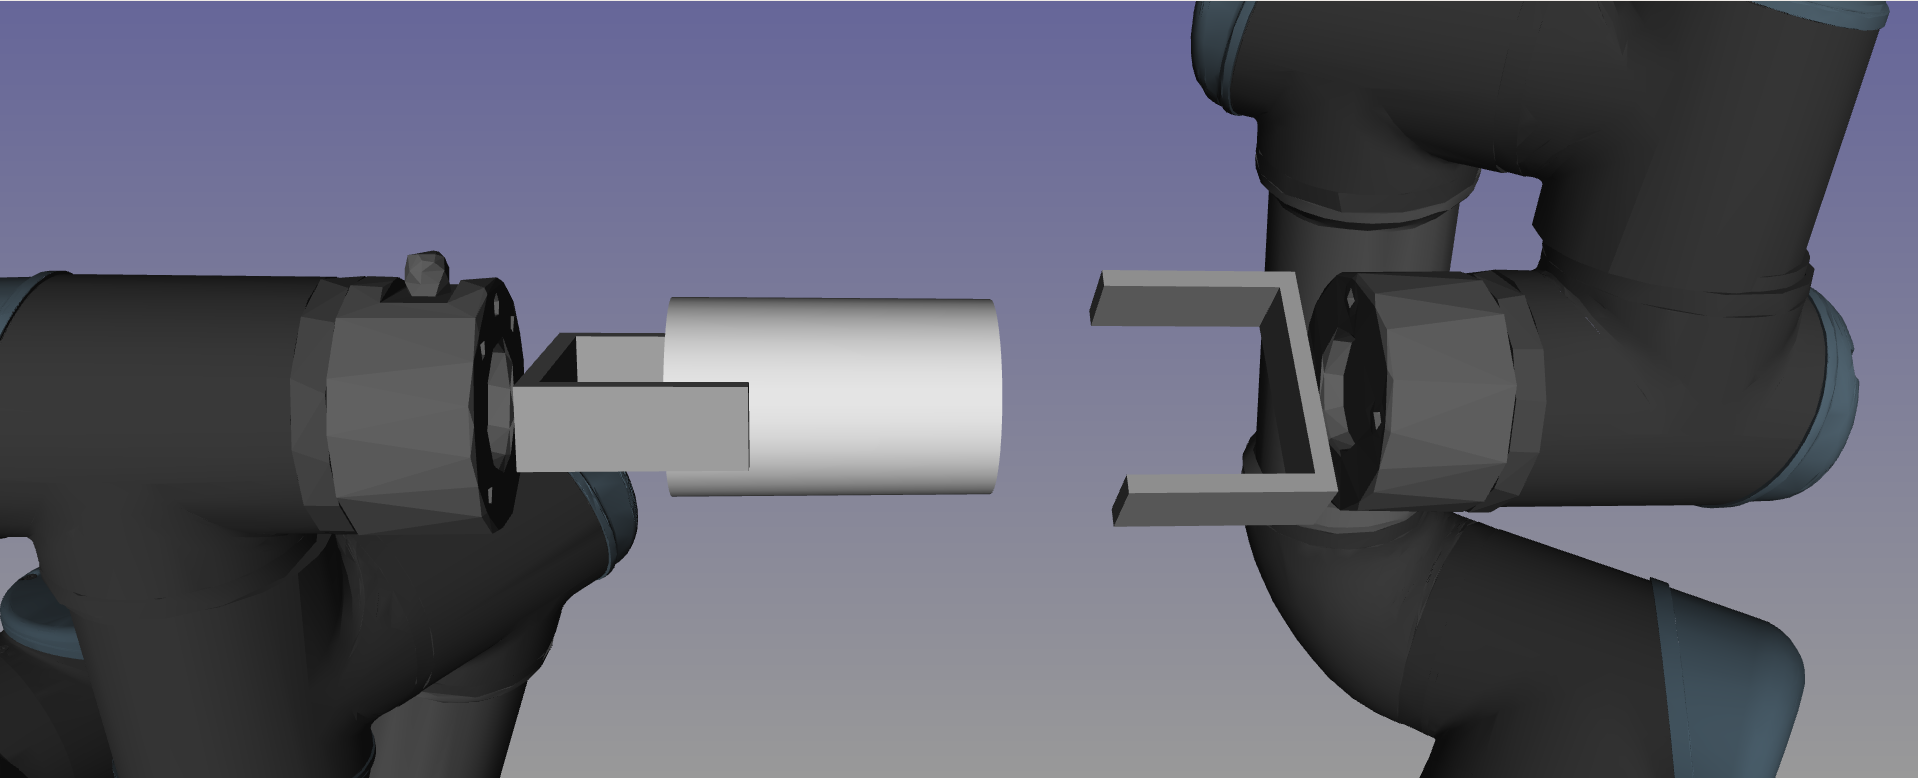
\includegraphics[width=.8\linewidth]{figures/dual-grasp-pregrasp.png}
  \end{center}
  \caption{Along a transition where an object already grasped is grasped by
    an additional gripper, an intermediate waypoint state called
    \textit{pregrasp} (pg) is added. This intermediate state is represented by
    an hexagonal box. $\gripper{2} > \handle{2}|(1,\emptyset)$ means that
    gripper 2 is going to grasp handle 2 from the state where gripper 1 grasps
    handle 1. The constraints associated to this waypoint state are the
    constraints of the state with the least active grasps (here $(1,\emptyset)$)
    and the pregrasp constraint corresponding to the grasp that is added in
    the node with the most active grasps (here $pregrasp_{22}$). The transition
    constraints are the same for all transitions (in red) and the same as
    the loop transition of the state with the least active grasps (in blue: here
    $grasp_{11}$ and $grasp_{11}/comp$).}
  \label{fig:pregrasp-grasp}
\end{figure}
\begin{figure}
  \centerline {
    \parbox {.69\linewidth} {
      \def\svgwidth {\linewidth}
      {
        \graphicspath{{./figures/}}
        \input {figures/placement-waypoints.pdf_tex}
      }
    }
    \parbox {.3\linewidth} {
      \begin {tabular}{c}
      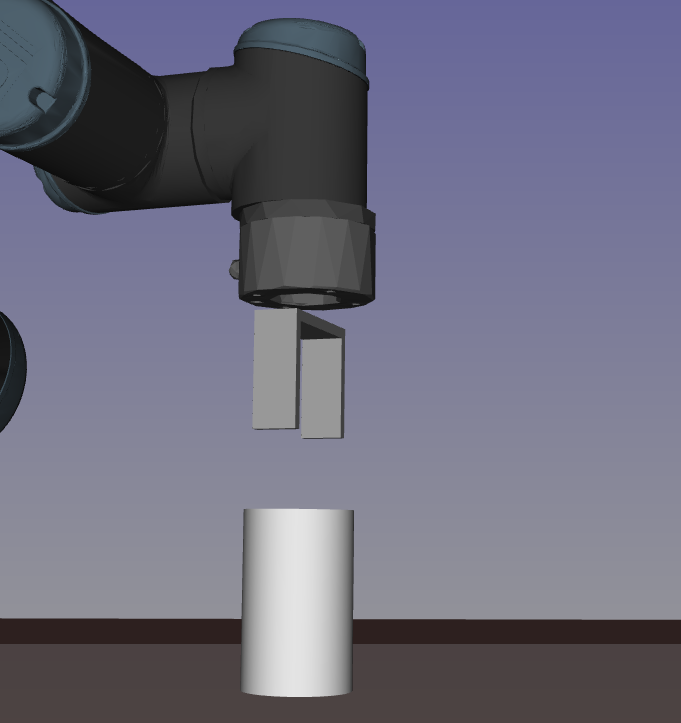
\includegraphics [width=.9\linewidth] {figures/placement-pregrasp-ur3.png}\\
      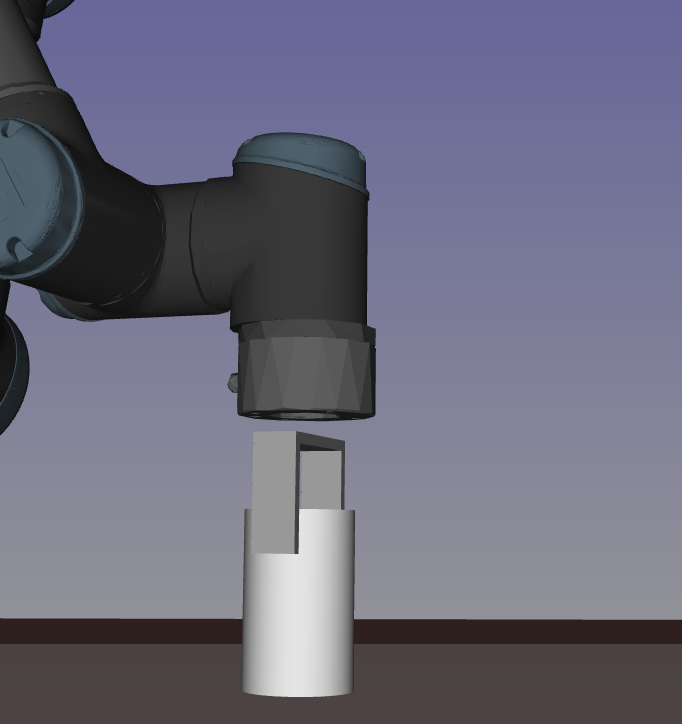
\includegraphics [width=.9\linewidth] {figures/placement-grasp-ur3.png}\\
      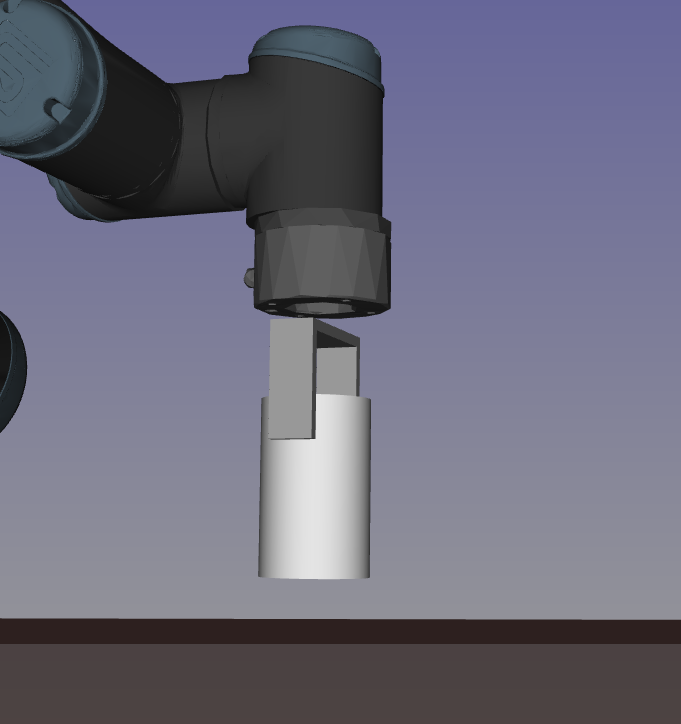
\includegraphics [width=.9\linewidth] {figures/placement-preplace-ur3.png}\\
      \end{tabular}
    }
  }
  \caption{Along a transition where an object in placement is grasped
    by a gripper, we add three waypoint states called
    \textit{pregrasp} (pg) where the gripper is above the object,
    \textit{grasp-placement} (gp) where the object is grasped but
    still in placement and \textit{preplacement} (pp) where the object
    is grasped above the contact surface. All transitions between the
    state with the least active grasps and the waypoint $gp$ have the
    same constraints as the loop transition of the state with the
    least active grasps (here: $place_1$ and $place_1/comp$ in
    blue). All transitions between the waypoint state $gp$ and the
    state with the most active grasps have the same constraints as the
    loop transition of the state with the most active grasps (here: $grasp_{11}$
    and $grasp_{11}/comp$ in red).}
  \label{fig:pregrasp-placement}
\end{figure}

A prehensile manipulation motion contains by definition configurations that are in contact:
\begin{itemize}
\item between gripper and object during grasp,
\item between object and contact surface when the object lies in a stable pose.
\end{itemize}
Contacts are difficult to handle by classical collision detection libraries and are often considered as collisions. To overcome this issue, we keep the gripper open during grasp, and objects slightly above contact surfaces in stable poses.

However even with these simple tricks, solution paths to a manipulation problem need to come close to collision, raising the well-known issue of narrow passages.

To cope with this issue, we define intermediate states in the
constraint graph called waypoint states. These states are inserted
between the regular states of the constraint graph. They require some prior
definitions.

\begin{definition}\label{def:pregrasp}\textbf{pregrasp}
  A \emph{pregrasp} is a numerical constraint $h$ over $\CS$, defined by
  \begin{itemize}
  \item a gripper $\gripper$,
  \item a handle $\handle$.
  \item a non-negative real number $\Delta$.
  \end{itemize}
  Let $\bar{h}$ be the smooth mapping from $\CS$ to $\reals^6$ that maps to any configuration $\conf$ of the system, the expression
  \begin{equation}\label{eq:barh-pregrasp}
    \bar{h}(\conf) = \log_{\reals^3\times SO(3)}\left(\gripper^{-1}(\conf) \handle(\conf)\right) - \left(\Delta\, 0\, 0\, 0\, 0\, 0\right)^T.
  \end{equation}
  $h(\conf)$ is obtained by extracting from $\bar{h}$ the components the values of which are \true in the handle flag.
\end{definition}
Note that when this constraint is satisfied, the handle is translated
along $x$ axis by distance $\Delta$ compared to a configuration
satisfying the grasp constraint. The value of $\Delta$ depends on the geometry
of the gripper and object. Clearance values are associated to the handle: $cl_{o}$ and to the gripper: $cl_{g}$. $\Delta$ is defined as $cl_{o}+cl_{g}$. The
clearance parameters are part of the definition of the gripper and handle and
are stored in SRDF files.

\begin{definition}\label{def:preplacement}\textbf{preplacement}
  A preplacement is a numerical constraint $h$ over $\CS$, defined by
  \begin{itemize}
  \item $(o_i)_{i\in I}$ a set of convex polygons attached to an object,
  \item $(f_j)_{j\in J}$ a set of convex polygons attached to the environment or to a mobile part of a robot that can receive objects (mobile robot for example),
  \item a non-negative real number $\Delta$.
  \end{itemize}
  with the same notation as in Section~\ref{subsec:placement}, we define $i$ and
  $j$ as the indices that minimize $d(f_j,o_i)$~
  (Equation~(\ref{eq:contact-distance})), and
  \begin{equation}\label{eq:convex-shape-contact-hbar-preplacement}
    \bar{h}(\conf) = \log_{\reals^3\times SO(3)} \left(f_{j}(\conf)^{-1}o_i(\conf)\right) + \left(\Delta\,0\,0\,0\,0\,0\right)^T
  \end{equation}
  The left hand side of the preplacement constraint is defined by Equation~
  (\ref{eq:convex-shape-contact}).
\end{definition}
Note that when this constraint is satisfied, the object is translated of a
distance $\Delta$ along the normal to the contact surface.

We denote by
\begin{itemize}
\item $pregrasp_{ij}\ i\in\{1,\cdots,\ngrippers\}\ j\in\{1,\cdots,\nhandles\}$ the pregrasp constraint of handle $j$ by gripper $i$,
\item $preplace_{i}\ i\in\{1,\cdots\nobjects\}$ the preplacement constraint of object $i$.
\end{itemize}

We replace the transitions of the constraint graph defined in
Section~\ref{subsec:constraint graph} by a sequence of intermediate
states and transitions as follows.

Following definition~\ref{def:neighboring-states}, if two states $\state_1$
and $\state_2$ are neighbors, one of them contains an additional grasp with
respect to the other one. Without loss of generality, let us consider that
$\state_2$ contains the additional grasp $\grasp{\gripper_i}{\handle_j}$,
$i\in\{1,\cdots\ngrippers\}$, $j\in\{1,\cdots\nhandles\}$. Then there are two
cases:
\begin{enumerate}
\item the object handle $\handle_j$ belongs to is already grasped in state
  $\state_1$, or
\item the object handle $\handle_j$ belongs to is in placement is
  state $\state_1$.
\end{enumerate}
In case 1, we replace the transitions between $\state_1$ and $\state_2$ by an additional waypoint state and four waypoint transitions as explained in Figure~\ref{fig:pregrasp-grasp}.

In case 2, we replace the transitions between $\state_1$ and $\state_2$ by three additional waypoint states and eight waypoint transitions as explained in Figure~\ref{fig:pregrasp-placement}.

\begin{figure}
  \centerline{
    \def\svgwidth {\linewidth}
      {\tiny
       \graphicspath{{./figures/}}
       \input {figures/waypoint-graph.pdf_tex}
    }
  }
  \caption{Structure of the constraint graph corresponding to the
    system in Section~\ref{subsec:ur3-cylinder} after inserting
    waypoint transitions.  Waypoint transitions starting from/going to
    $(\emptyset,\emptyset)$ contain three waypoint states. All other
    waypoint transitions contain one waypoint state.}
\end{figure}

\begin{figure}
  \begin{center}
    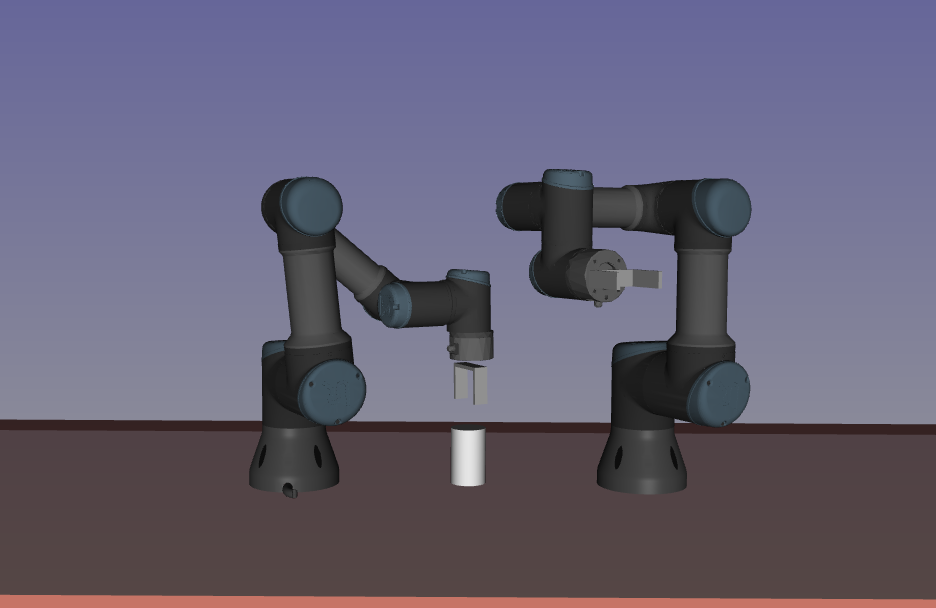
\includegraphics[width=.75\linewidth]{figures/example-q-wp-1.png}
    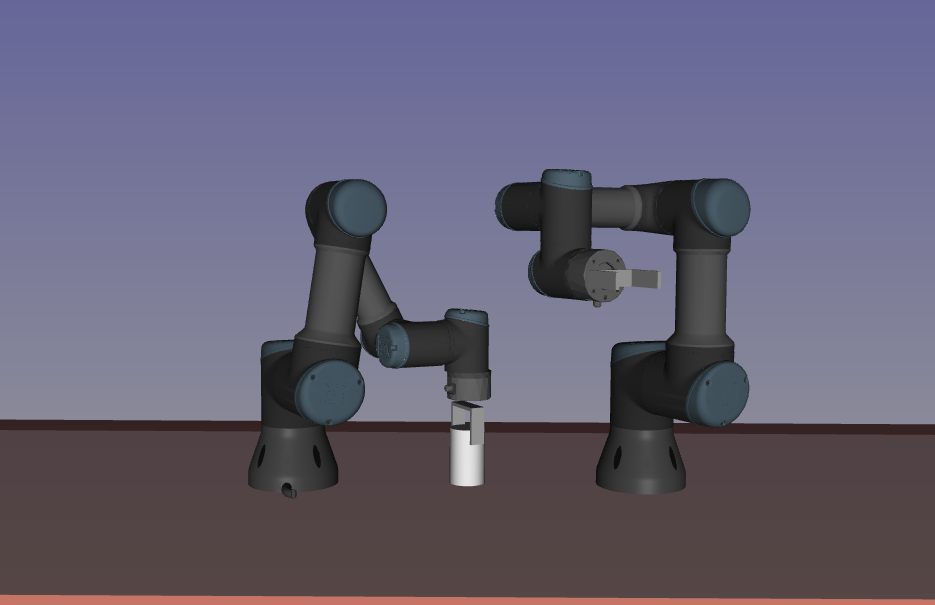
\includegraphics[width=.75\linewidth]{figures/example-q-wp-2.png}
    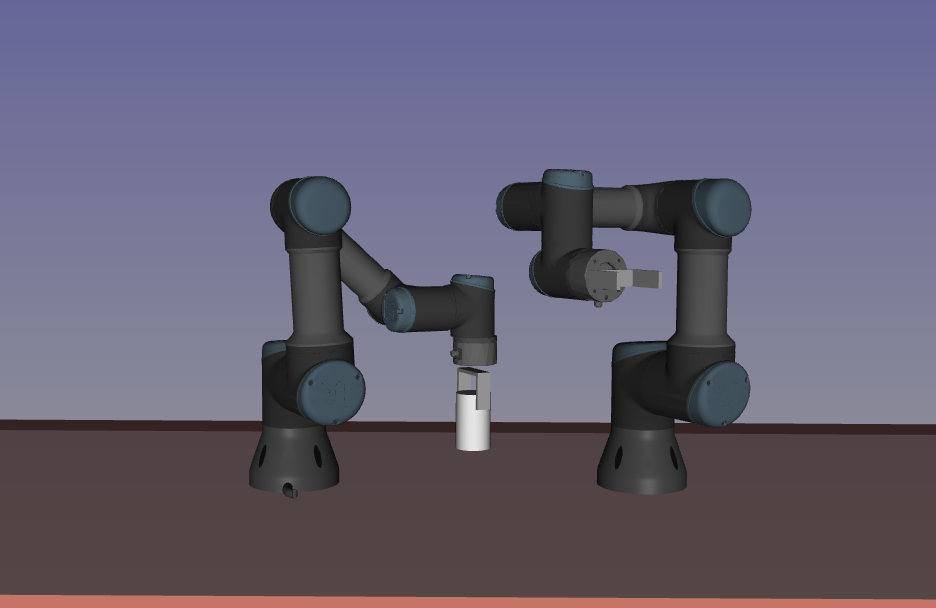
\includegraphics[width=.75\linewidth]{figures/example-q-wp-3.png}
  \end{center}
  \caption{Example of extension along the waypoint transition between states
    $(\emptyset,\emptyset)$ and $(1,\emptyset)$. Each picture represents a
    waypoint. The last waypoint is in state $(1,\emptyset)$. $\conf_{near}$
    and $\conf_{rand}$ are the same as in Figure~\ref{fig:MRRT-extension}.}
  \label{fig:MRRT-extension-wp}
\end{figure}

\paragraph{Construction of a path along a waypoint transition} Function
{\scriptsize EXTEND} in Algorithm~\ref{algo:M-RRT} builds a path along a
transition from an initial configuration by projecting the configuration
onto the sub-manifold defined by the goal state constraints and by the
transition constraints. The right hand side of the transition constraint is
first initialized with the initial configuration.

A waypoint transition builds a path by defining a sequence of configurations
that belong to the intermediate waypoint states, each waypoint is obtained by
projecting the previous waypoint onto the corresponding manifold.
Figure~\ref{fig:MRRT-extension-wp} proposes an example of extension along
edge $(\emptyset,\emptyset)\rightarrow(1,\emptyset)$ from configuration
$\conf_{near}$ (Figure~\ref{fig:MRRT-extension} middle). The edge contains three
waypoints. The random configuration $\conf_{rand}$ is displayed in
Figure~\ref{fig:MRRT-extension} top. Table~\ref{table:waypoints} lists the
waypoint configurations that are produced when extending $\conf_{near}$ toward
$\conf_{rand}$, and the constraints applied to compute these configurations.
\begin{table}
{
\begin{tabular} {|l|l|}
  \hline
  $\conf_{near}$ &
  \begin{tabular}{l} \textbf{in state} $(\emptyset,\emptyset)$ \\
  \end{tabular}\\
  \hline
  $\conf_1$ &
  \begin{tabular}{l} \textbf{waypoint state} $\gripper{1}>\handle{1}|(\emptyset,\emptyset)|pg$ \\
    \textbf{in state} $(\emptyset,\emptyset)$ \\
    \textbf{constraints} \\
    {\color{blue}$place_1(\conf)=0$} \\
    {\color{blue}$place_1/comp(\conf) = place_1/comp(\conf_{near})$} \\
    $pregrasp_{11}(\conf) = 0$ \\
    \textbf{solver initialized with} $\conf_{rand}$
  \end{tabular}\\
  \hline
  $\conf_2$ & 
  \begin{tabular}{l}
    \textbf{waypoint state} $\gripper{1}>\handle{1}|(\emptyset,\emptyset)|gp$ \\
    \textbf{in states} $(\emptyset,\emptyset)$ and $(1,\emptyset)$ \\
    \textbf{constraints} \\
    {\color{blue}$place_1(\conf)=0$} \\
    {\color{blue}$place_1/comp(\conf) = place_1/comp(\conf_{near})$} \\
    $grasp_{11}(\conf) = 0$ \\
    \textbf{solver initialized with} $\conf_{1}$
  \end{tabular} \\
  \hline
  $\conf_{target}$ &
  \begin{tabular}{l}
    \textbf{waypoint state} $\gripper{1}>\handle{1}|(\emptyset,\emptyset)|pp$ \\
    \textbf{in state} $(1,\emptyset)$ \\
    \textbf{constraints} \\
    {\color{blue}$grasp_{11}(\conf)=0$} \\
    {\color{blue}$grasp_{11}/comp(\conf) = grasp_{11}/comp(\conf_{2})$} \\
    $preplace_{1}(\conf) = 0$\\
    \textbf{solver initialized with} $\conf_{2}$
  \end{tabular}\\
  \hline
\end{tabular}
\caption{Waypoint configurations computed along edge $(\emptyset,\emptyset)\rightarrow(1,\emptyset)$.
  The resulting path between $\conf_{near}$ and $\conf_{target}$ is a concatenation
  of constrained linear interpolation. Constraints applied between a waypoint
  and its predecessor are shown in blue.}
\label{table:waypoints}
}
\end{table}
\paragraph{Implementation} From an implementation point of view, Class
\href{https://gepettoweb.laas.fr/hpp/hpp-manipulation/doxygen-html/classhpp_1_1manipulation_1_1graph_1_1WaypointEdge.html}{\texttt{WaypointEdge}} derives from class \href{https://gepettoweb.laas.fr/hpp/hpp-manipulation/doxygen-html/classhpp_1_1manipulation_1_1graph_1_1Edge.html}{\texttt{Edge}}. The waypoint configurations are computed by method\\ \texttt{generateTargetConfig} that is specialized in
Class\\ \texttt{WaypointEdge}.

Note that waypoint states are internal to waypoint edges and are not known by
the constraint graph when determining to which state a configuration belongs
(Algorithm~\ref{algo:M-RRT} lines~17 and 23) and when visiting the states of the
constraint graph (Algorithm~\ref{algo:M-RRT} line~8).

\section{Humanoid Path Planner}\label{sec:humanoid-path-planner}

In this section, we describe in more details the software platform
\href{https://humanoid-path-planner.github.io/hpp-doc}{Humanoid Path
  Planner} that implements the concepts and algorithms of the previous
sections.

Humanoid Path Planner is a collection of standard software packages that depend
on each other. The main packages are the following:
\begin{itemize}
\item \texttt{hpp-fcl} a modified version of \href{https://github.com/flexible-collision-library/fcl}{\texttt{fcl}}. The main additional features are the following:
  \begin{itemize}
  \item computation of a lower bound of the distance when testing collision
    between two objects. This is required for continuous collision detection,
  \item security margins in collision checking,
  \end{itemize}
\item \href{https://stack-of-tasks.github.io/pinocchio}{\texttt{pinocchio}}~\cite{pinocchio} a library computing forward kinematics and dynamics for multi-body kinematic chains,
\item \texttt{hpp-constraints} a library that implements numerical constraints
  and solvers,
\item \texttt{hpp-core} a library that implements most of the concepts relative
  to motion planning. The main features are
  \begin{itemize}
  \item abstraction of paths in configuration spaces and some implementations,
  \item abstraction of path planning and path optimization and some implementations,
  \item abstraction of steering methods and some implementations,
  \item roadmaps,
  \item validation of configurations and paths, {\color{blue} notice that this
    includes an implementation of continuous collision checking first proposed
    by Schwarzer \textit{et al}~\cite{SchSahLat2004}.}
  \end{itemize}
\item \texttt{hpp-manipulation} a library that implements manipulation
  problems and manipulation planning with
  \begin{itemize}
    \item composite kinematic chains composed of the robots and objects,
    \item the constraint graph,
    \item M-RRT algorithm,
  \end{itemize}
\item \texttt{hpp-manipulation-urdf} an extension of the SRDF parser to retrieve
  information relative to objects, like the definition of grippers, handles, and
  contact surfaces.
\end{itemize}
An HPP session consists of a standalone executable \texttt{hppcorbaserver}
that implements CORBA services. These services can be extended via a plugin
system. The application can then be controlled via python script or C++ code.
CORBA clients are provided in python and C++. The packages implementing CORBA
clients and servers are
\begin{itemize}
\item \texttt{hpp-corbaserver} for canonical path planning problems, and
\item \texttt{hpp-manipulation-corba} for manipulation problems. This
latter package also provides an implementation of the automatic constraint graph
construction in python.
\end{itemize}
The environment used for path planning as well as the paths computed can be
displayed using \texttt{gepetto-gui} through packages
\begin{itemize}
  \item\texttt{gepetto-viewer},
  \item\texttt{gepetto-viewer-corba}, and
  \item\texttt{hpp-gepetto-viewer}.
\end{itemize}

\subsection{Virtual machine}

A virtual docker image can be downloaded to run, test and replicate the
examples described in the next sections. An archive is provided with this paper.
Decompress the archive and follow instructions in the README file.

\subsection{Experimental results}\label{sec:benchmarks}

In this section, we report on several experimental results obtained
with HPP software on constrained motion planning and on manipulation
planning problems. The raw data can be found in
\href{https://github.com/humanoid-path-planner/hpp_benchmark/tree/v4.10.0/2020-07-23}{\texttt{hpp\_benchmark}} package. Here we present only a few test cases.
The benchmarks are run 20 times each on an Intel Core i7 at 2.60 GHz, with 32 Gigabytes of RAM and 3 Gigabytes of cache memory. For each test case, we report the minimum, maximum, mean and standard deviation of the time of computation on the one hand, and of the number of nodes in the roadmap built to solve the problem on the other hand.

\subsubsection{Constrained motion planning}

\begin{figure}
  \begin{center}
    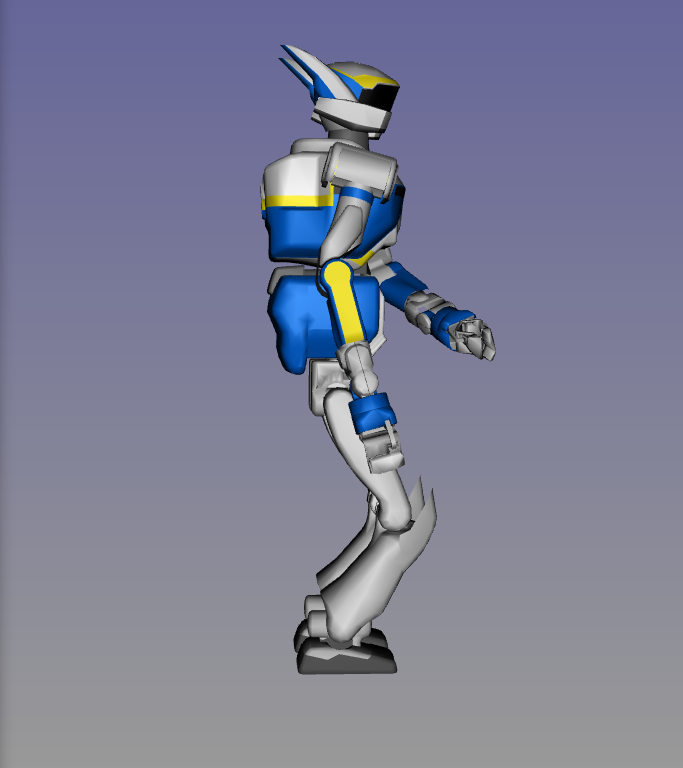
\includegraphics[width=.49\linewidth]{figures/hrp2-q-init.png}
    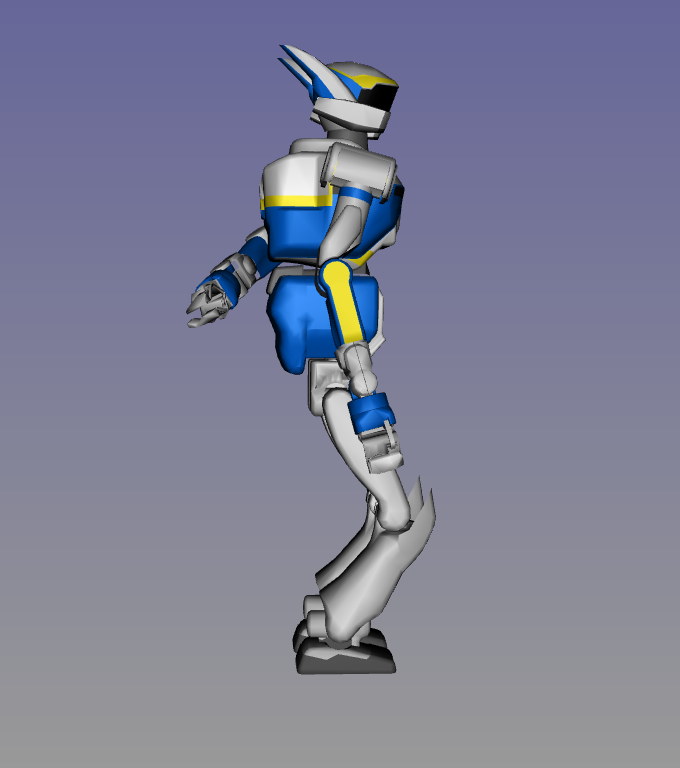
\includegraphics[width=.49\linewidth]{figures/hrp2-q-goal.png}
  \end{center}
  \caption{Constrained motion planning for HRP-2 humanoid robot sliding on the ground in quasi-static equilibrium: the feet should stay horizontal with a fixed relative position and the center of mass should project between the feet. The initial configuration is shown on the left. The goal configuration is shown on the right. The algorithm is a constrained RRT close to the one described in {\color{blue}Dalibard \textit{et al}}~\cite{DalNakLamLau2009}}.
  \label{fig:benchmark-hrp2}
\end{figure}
One test case concerns constrained motion planning. The robot is an HRP-2 humanoid robot in quasi-static equilibrium that can slide on the ground ( {\color{blue}Figure~\ref{fig:benchmark-hrp2}} ). This type of motion can be post-processed into a walking motion using the method described in {\color{blue}Dalibard \textit{et al}}~\cite{dalibard:hal-00654175}. The results are displayed in Table~\ref{tab:benchmark-hrp2}.
\begin{table}
  \begin{center}
  \begin{tabular}{|l|l|l|l|l|}
    \hline
    & min & max & mean & std dev \\
    \hline
    time (s) & 0.03 & 11.64 & 1.32 & 2.55 \\
    nodes & 4 &  136 & 32.40 & 30.72\\
    \hline
  \end{tabular}
  \end{center}
  \caption{Experimental results for HRP-2 sliding on the ground {\color{blue}(36 degrees of freedom)}: time of computation and number of nodes.}
  \label{tab:benchmark-hrp2}
\end{table}

\subsubsection{Manipulation planning}

In this section, we present some experimental results of manipulation planning
problems obtained with M-RRT algorithm described in Section~\ref{sec:manipulation-planning}.

\begin{figure}
  \begin{center}
    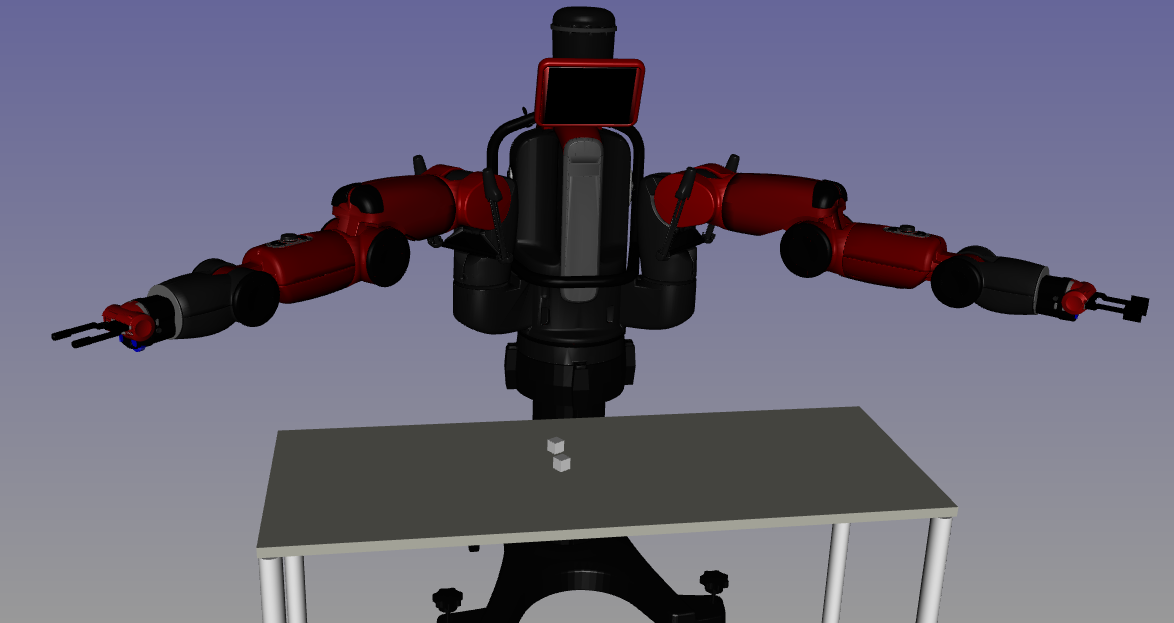
\includegraphics[width=\linewidth]{figures/baxter-manipulation-boxes}
  \end{center}
  \caption{Manipulation problem with Baxter robot manipulating two small boxes. The robot is requested to swap the boxes.}
  \label{fig:baxter-manipulation-boxes}
\end{figure}

\begin{table}
  \begin{center}
  \begin{tabular}{|l|l|l|l|l|}
    \hline
    & min & max & mean & std dev \\
    \hline
    time (s) & 0.84 & 15.60 & 7.60 & 4.48 \\
    nodes & 23 &  375 & 176.15 & 108.54 \\
    \hline
  \end{tabular}
  \end{center}
  \caption{Experimental results for Baxter robot manipulating two boxes on a table {\color{blue}(31 degrees of freedom)}.}
  \label{tab:baxter-manipulation-boxes}
\end{table}

The first test case features robot Baxter manipulating two boxes on a table (see Figure~\ref{fig:baxter-manipulation-boxes}). The boxes are swapped between the initial and final configurations. The robot has two grippers and each box is equipped with a handle. The constraint graph thus contains 7 nodes. The experimental results are displayed in Table~\ref{tab:baxter-manipulation-boxes}.

\begin{figure}
  \begin{center}
    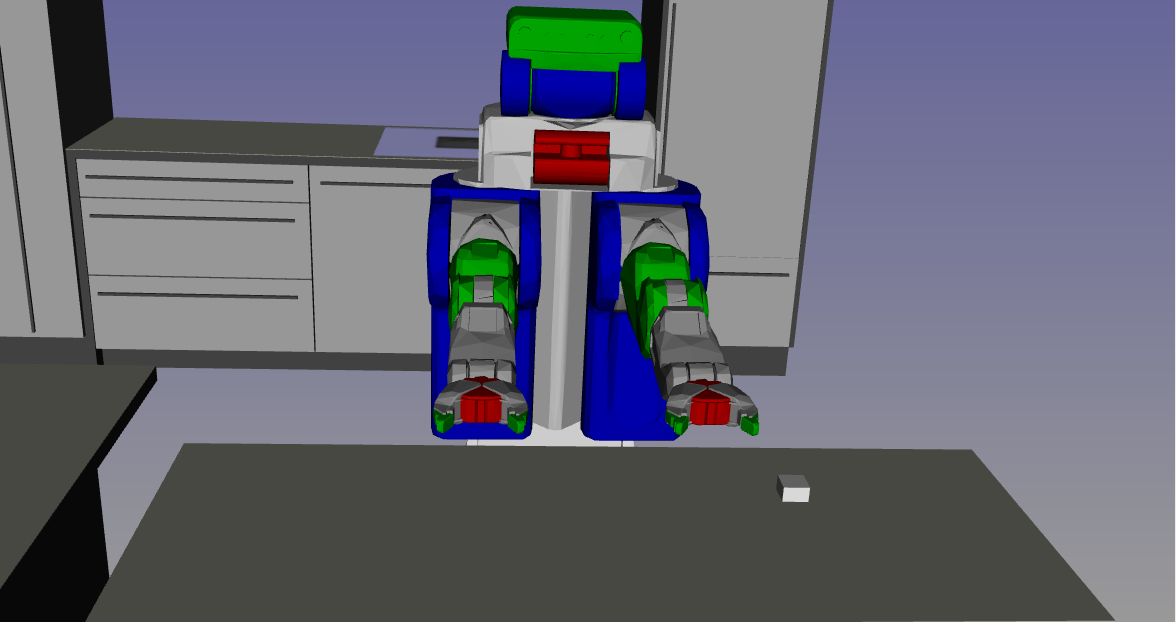
\includegraphics[width=\linewidth]{figures/pr2-manipulation-two-hands-init.png}
    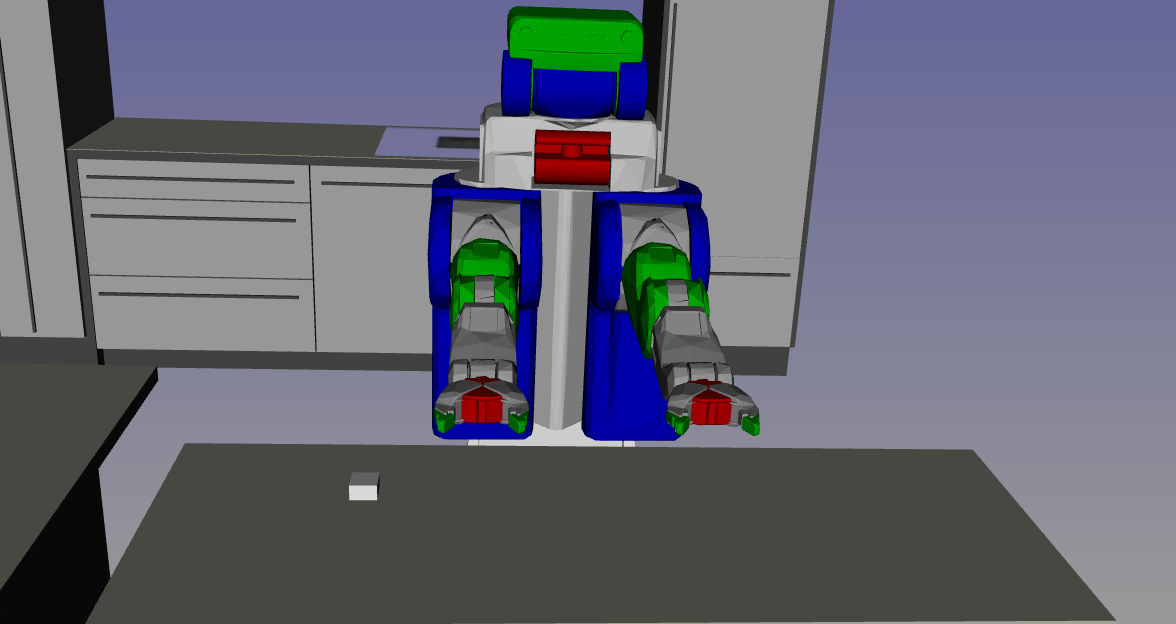
\includegraphics[width=\linewidth]{figures/pr2-manipulation-two-hands-goal.png}    
  \end{center}
  \caption{Manipulation planning problem with PR-2 robot manipulating a box. The robot needs to flip the box upside down from an initial pose (top) to a goal pose (bottom).}
  \label{fig:pr2-manipulation-two-hands}
\end{figure}

\begin{table}
  \begin{center}
  \begin{tabular}{|l|l|l|l|l|}
    \hline
    & min & max & mean & std dev \\
    \hline
    time (s) & 0.92 & 9.62 & 3.30 & 2.47 \\
    nodes & 6 &  111 & 32.90 & 31.63 \\
    \hline
  \end{tabular}
  \end{center}
  \caption{Experimental results for PR-2 robot manipulating a box on a table
     {\color{blue}(39 degrees of freedom)}.}
  \label{tab:pr2-manipulation-two-hands}
\end{table}

The second test case features robot PR-2 manipulating a box on a table. The robot is requested to flip the box upside down from an initial pose to a goal pose as represented in Figure~\ref{fig:pr2-manipulation-two-hands}. The robot is equipped with two grippers, the box is equipped with two handles. The constraint graph contains 7 nodes. Table~\ref{tab:pr2-manipulation-two-hands} shows the experimental results.


\begin{figure}
  \begin{center}
    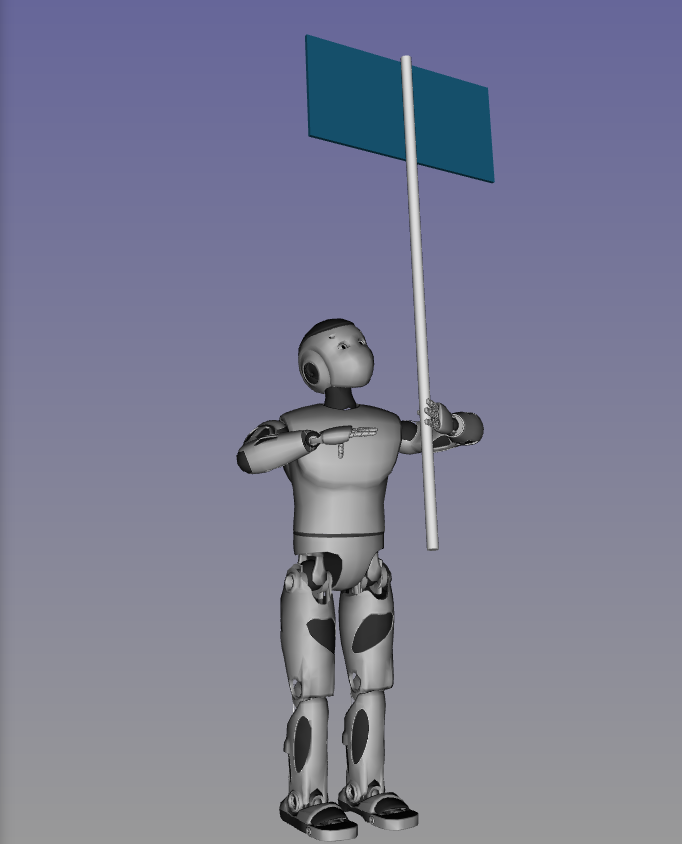
\includegraphics[width=.49\linewidth]{figures/romeo-placard-init.png}
    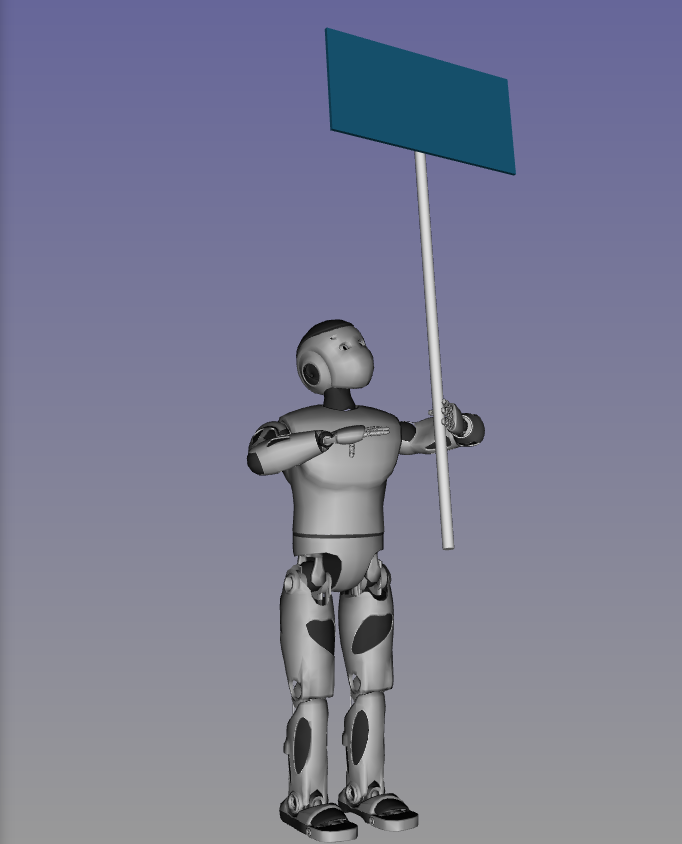
\includegraphics[width=.49\linewidth]{figures/romeo-placard-goal.png}    
  \end{center}
  \caption{Manipulation planning problem with Romeo robot manipulating a placard. The robot needs to flip the placard by 180 degrees from an initial pose (left) to a goal pose (right), keeping balance.}
  \label{fig:romeo-placard}
\end{figure}

\begin{table}
  \begin{center}
  \begin{tabular}{|l|l|l|l|l|}
    \hline
    & min & max & mean & std dev \\
    \hline
    time (s) & 4.64 & 554.18 & 151.49 & 158.64 \\
    nodes & 27 &  2448 & 610.45 & 662.83 \\
    \hline
  \end{tabular}
  \end{center}
  \caption{Experimental results for Romeo robot manipulating a placard
    {\color{blue}(67 degrees of freedom)}.}
  \label{tab:romeo-placard}
\end{table}

The third test case features Humanoid Robot Romeo manipulating a placard. The
robot is requested to rotate the placard by 180 degrees. The robot is equipped
with two grippers and the placard with two handles. Each handle is associated
to a single gripper. The number of states of the constraint graph is thus 3.

\begin{figure}
  \begin{center}
    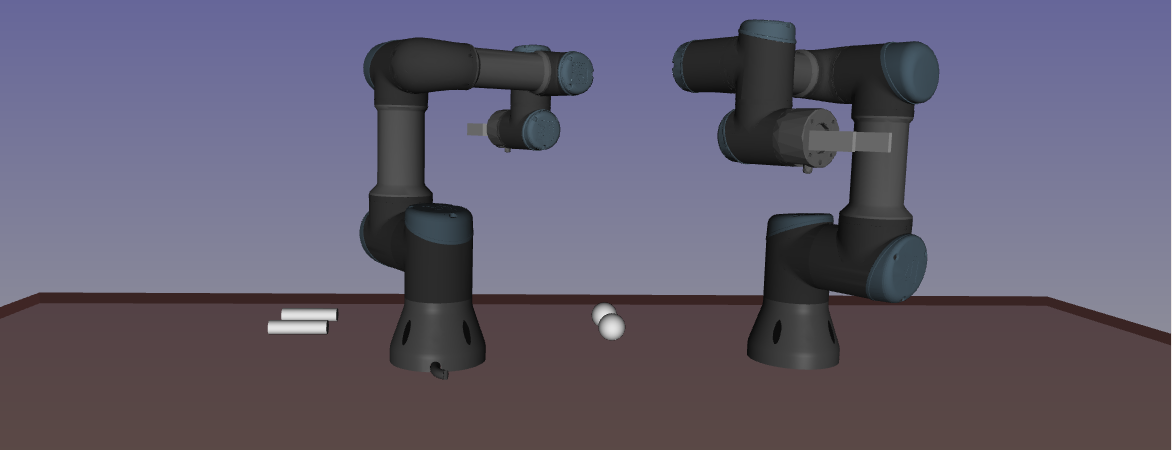
\includegraphics[width=\linewidth]{figures/construction-set-init.png}
    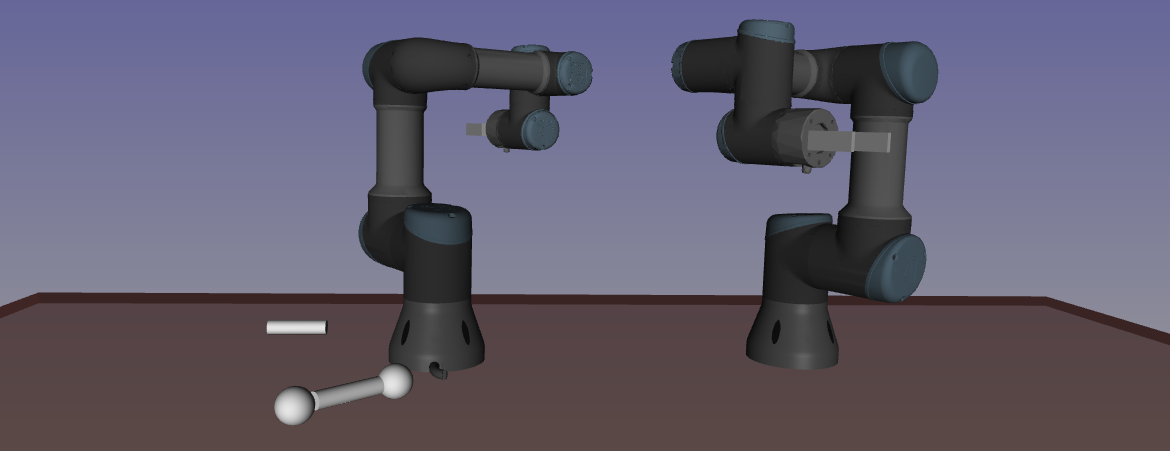
\includegraphics[width=\linewidth]{figures/construction-set-goal.png}    
  \end{center}
  \caption{Construction set: two robots are requested to assemble magnetic
    spheres on a cylinder from an initial configuration (top) to a goal state
    (bottom).}
  \label{fig:construction-set}
\end{figure}

\begin{table}
  \begin{center}
  \begin{tabular}{|l|l|l|l|l|}
    \hline
    & min & max & mean & std dev \\
    \hline
    time (s) & 0.20 & 214.22 & 17.11 & 45.84 \\
    nodes & 10 &  39 & 14.70 & 6.48 \\
    \hline
  \end{tabular}
  \end{center}
  \caption{Experimental results for construction set assembly
    {\color{blue}(36 degrees of freedom)}.}
  \label{tab:construction-set}
\end{table}

In the three previous test cases, the constraint graph was automatically built
following Algorithm~\ref{algo:constraintGraphFactory}. If the number of grippers
and handles increases, the number of states in the constraint may increase very
quickly. However using python bindings, it is possible to define constraint
graphs with only the necessary states. We now present a test case that
illustrates this possibility. The system is represented in Figure~\ref{fig:construction-set}.

In this example, an operator provides the sequence of actions (transitions)
the system needs to go through:
\begin{enumerate}
\item robot 1 grasps sphere 1,
\item robot 2 grasps cylinder 1,
\item robot 1 sticks sphere 1 on cylinder 1,
\item robot 1 releases sphere 1,
\item robot 1 grasps sphere 2,
\item robot 1 sticks sphere 2 on cylinder 1,
\item robot 1 releases sphere 2,
\item robot 2 puts cylinder 1 on the ground.
\end{enumerate}
From this sequence of actions, the sequence of states visited is
computed and only those states (9 in total) are built in the
constraint graph. Then, a sequence of sub-goals in the successive
states is computed, in such a way that each sub-goal is accessible by
the previous one (on the same leaf of the corresponding transition
foliation). The sub-goals are then linked by running a constrained visibility
PRM algorithm \cite{SimLauNis00} on each leaf. The python code can be found
on \href{https://github.com/humanoid-path-planner/hpp_benchmark/blob/master/2020-07-23/construction-set/script.py}{github.com}.

Figure~\ref{fig:construction-set} displays the initial configuration and the
goal state. Table~\ref{tab:construction-set} shows the experimental results.

\subsubsection{Influence of waypoint transitions}

\begin{figure}
  \begin{center}
    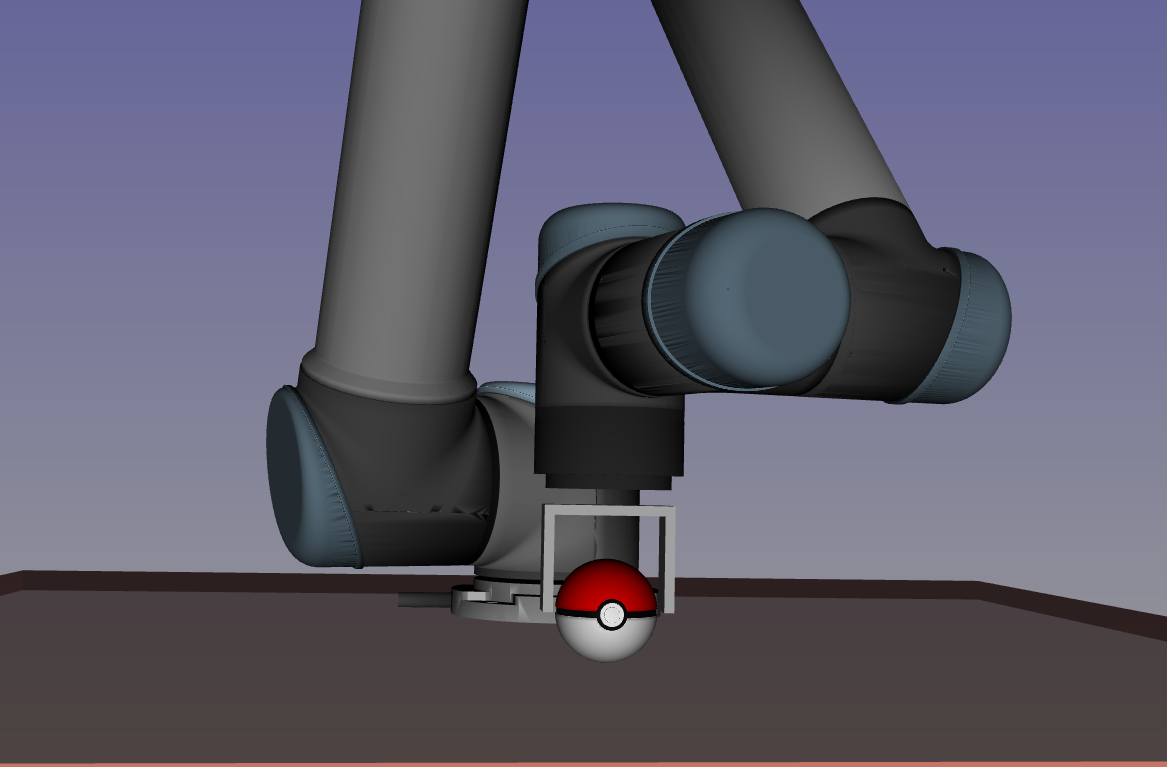
\includegraphics[width=\linewidth]{figures/ur5-grasps-pokeball.png}
  \end{center}
  \caption{UR-5 robot manipulating a ball lying on a plane. The robot is requested to pick the ball and place it a few centimeters aside.}
  \label{fig:ur5-pokeball}
\end{figure}

\begin{table}
  \begin{center}
  \begin{tabular}{|l|l|l|l|l|}
    \hline
    & min & max & mean & std dev \\
    \hline
    with waypoints&&&&\\
    time (s) & 0.01 & 0.49 & 0.12 & 0.14 \\
    nodes & 4 &  30 & 9.75 & 7.26\\
    \hline
    without waypoints&&&&\\
    time (s) & 4.15 & 73.53 & 26.24 & 17.07 \\
    nodes & 97 &  1609 & 711.55 & 407.98\\
    \hline
  \end{tabular}
  \end{center}
  \caption{UR-5 manipulating a ball with and without waypoint transitions}
  \label{tab:waypoint}
\end{table}

All the previous experimental results have been obtained using
waypoint transitions as described in Section~\ref{subsec:waypoint}. We
now empirically show the positive effect of waypoints on the
efficiency of manipulation planning. For that, we run 20 times
Algorithm M-RRT on the same problem with and without waypoint
transitions.  The problem is defined by a UR-5 robot manipulating a
ball as shown in Figure~\ref{fig:ur5-pokeball}. The results are
reported in Table~\ref{tab:waypoint}. We can notice that for this
example, the waypoint transitions make the time of computation and the
number of nodes decrease by 2 orders of magnitude. This can be
explained by the fact that in grasp configurations, the gripper is
very close to the object and only a small part of the approaching
directions of the gripper toward the object leads to collision-free
paths. Waypoint states on the contrary are away from obstacles and
easier to reach. The transition between the pregrasp waypoint and the
grasp $\cap$ placement waypoint is always collision-free.

\subsubsection{Analysis}

The experimental results show that M-RRT is able to solve a variety of
manipulation problems including with a legged robot in quasi-static
equilibrium. No parameter tuning is required between the different problems. All
parameters are set to a default value for all test cases.

As for any random motion planning method, we observe a large standard
deviation within the 20 runs of each test case, both for the number of nodes
and for the time of computation.

We have also observed experimentally that the efficiency of M-RRT decreases
when
\begin{enumerate}
\item the number of states to visit to solve a problem increases,
\item the number of foliated states increases.
\end{enumerate}
For this reason, M-RRT is not able to solve the construction set
problem in a reasonable amount of time. However, it remains to our knowledge
the only algorithm in the literature able to solve a variety of
problems as large as those presented in this section.

\section{Conclusion and future work}

This paper presents a software platform aimed at prototyping and
solving a great variety of prehensile manipulation planning
problems. The platform provides an original algorithm M-RRT that is an
extension of RRT exploring the leaves of the foliations defined by the
manipulation constraints. The automatic insertion of waypoint states
makes the resolution more efficient and the resulting paths more
natural.

We think that this platform is a perfect basis for researchers who want to
develop and benchmark new manipulation planning algorithms. Note that some
on-going work in humanoid locomotion  \cite{tonneau-2018} is based on HPP.

To show the maturity of the project, we provide a docker image embarking the
software.

As a future work, we aim at working on general manipulation planning algorithms
that can handle use cases as diverse as those proposed in the benchmark section.
A good candidate is a generalization of RMR*~\cite{schmitt17icra}. We also aim at working on manipulation path optimization since paths computed by
random algorithms are too long to be applied on real robots as such.
